\chapter{Resultados y discusión}
En este capítulo se presentan las relaciones entre la cantidad de potencia transmitida por radiación (que es una potencia aprovechable para generar electricidad) y la cantidad de potencia transmitida por conducción (la cual no se puede aprovechar) para diferentes combinaciones de materiales de emisor y célula.\\\\
Para determinar estas relaciones se simula la transmisión de calor por conducción a través de un nano-espaciador, para luego extrapolar la cantidad de calor por conducción que se obtendría para un dispositivo de $1cm^2$ con distintas distribuciones de nano-espaciadores ($nº espaciadores/cm^2$, y se simula la transmisión de calor por radiación de campo cercano en un dispositivo de $1cm^2$. Las simulaciones se realizan con el emisor a una temperatura constante de 800\textdegree C y la célula a 25\textdegree C.
\begin{itemize}
	\item Primero se valida la simulación de CFD.
	\item Se presentan los resultados de las simulaciones de transmisión de calor por conducción y por radiación de campo cercano para diferentes combinaciones de materiales de emisor y célula, y la relación entre ambas simulaciones.
	\item Se estudia el número mínimo de espaciadores necesarios para soportar la carga de los emisores.
	\item Por último, se presentan los resultados de usar un nano-espaciador de $Si$ en vez de $SiO_2$ para emisores de $Si$ y $SS$.
\end{itemize}
%% COMPROBACIÓN DEL PROCEDIMIENTO DE EXTRACCIÓN DE RESULTADOS DE CFD
\section{Validación de las simulaciones de CFD}
Las simulaciones de CFD son validas al comprobarse que con ellas se obtienen los mismos resultados que el modelo analítico (ecuación \eqref{eq:conduccion}) cuando se imponen las mismas simplificaciones de dicho modelo, es decir, cuando se impone una conductividad térmica constante y altura del nano-espaciador de 1000nm.
\begin{equation}
Q=k\cdot \Delta T
\label{eq:conduccion}
\end{equation}
La conductividad térmica ($\sigma$) del $Si$ es 182.977 W/m\textdegree C y la del $SiO_2$ es 1.30067 W/m\textdegree C ambas a 25\textdegree C. De la simulación se extrae el flujo de calor del sistema y la temperatura media máxima y mínima de las superficies de contacto del nano-espaciador con los otros componentes del sistema.\\\\
La temperatura media máxima del nano-espaciador es 792.601\textdegree C, la temperatura media mínima del nano-espaciador es 32.3903\textdegree C y el flujo de calor es 0.00889793 W. Con los resultados de las temperaturas medias del nano-espaciador se obtiene un flujo de calor teórico de 0.00889905 W (obtenido mediante la ecuación \eqref{eq:conduccion}, siendo $k$ la conductancia térmica $k=\sigma \cdot A/L$), obteniéndose un error relativo aproximado del 0.0126\%, por lo tanto el procedimiento es apropiado para la obtención de los resultados de las simulaciones de transmisión de calor por conducción.
%%% SIMULACIONES DE TRANSMISIÓN DE CALOR POR CONDUCCIÓN EN CFD
\section{Resultados de las simulaciones para una nTPV de Si-SiO2-Si}
A continuación se estudian los efectos de la resistencia de contacto y la porosidad sobre un sistema sencillo compuesto por un emisor de $Si$ de 1 $mm$ lado y 0.2 $mm$ de altura con la cara superior a 800 \textdegree C, un nano-espaciador de 3 $\mu m$ de lado y una célula de $Si$ de las mismas dimensiones que el emisor con la cara inferior a 25\textdegree C.
\subsection{Efectos de la resistencia de contacto sobre la conducción}
La resistencia de contacto ($R_c$) usada es de unos $4\cdot 10^{-6} \ m^2 K/W$ \cite{nf_TPV_Pillars_SiO2} que es aplicada a la superficie superior del nano-espaciador que entra en contacto con la superficie inferior del emisor, solo se considera en dicha superficie porque el nano-espaciador será depositado sobre la superficie de la célula en la fase de fabricación, con lo cual la interfaz de con la célula se considera perfecta.
\begin{figure}[H]
	\centering
	\begin{subfigure}[b]{0.49\textwidth}
		\centering
		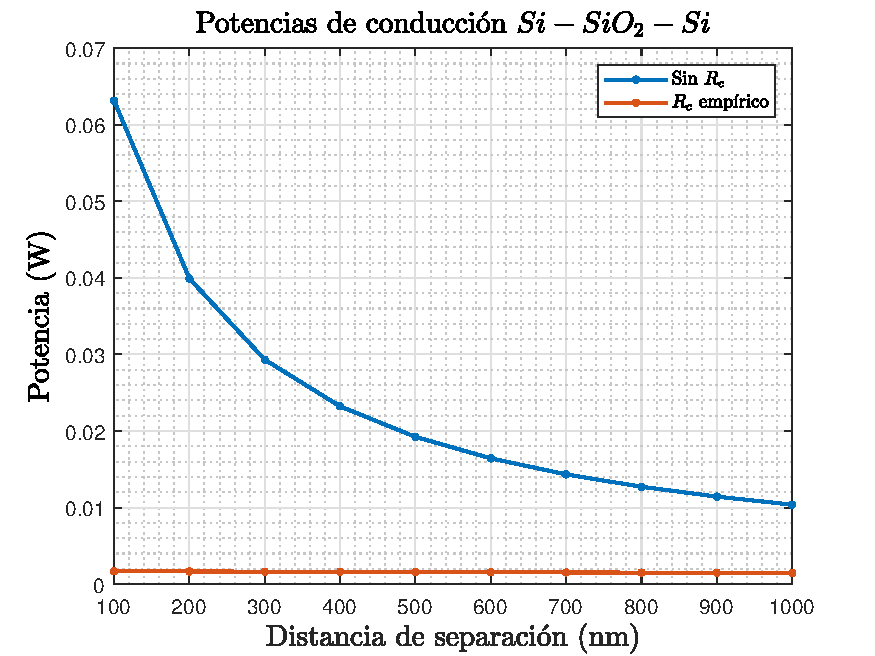
\includegraphics[width=1.0\textwidth]{figuras/Resultados/conduccion/pdf/Prc_SiSiO2Si.pdf}
		\caption{Potencias con y sin $R_c$}
		\label{fig:Prc_SiSiO2Si}
	\end{subfigure}
	\hfill
	\begin{subfigure}[b]{0.49\textwidth}
		\centering
		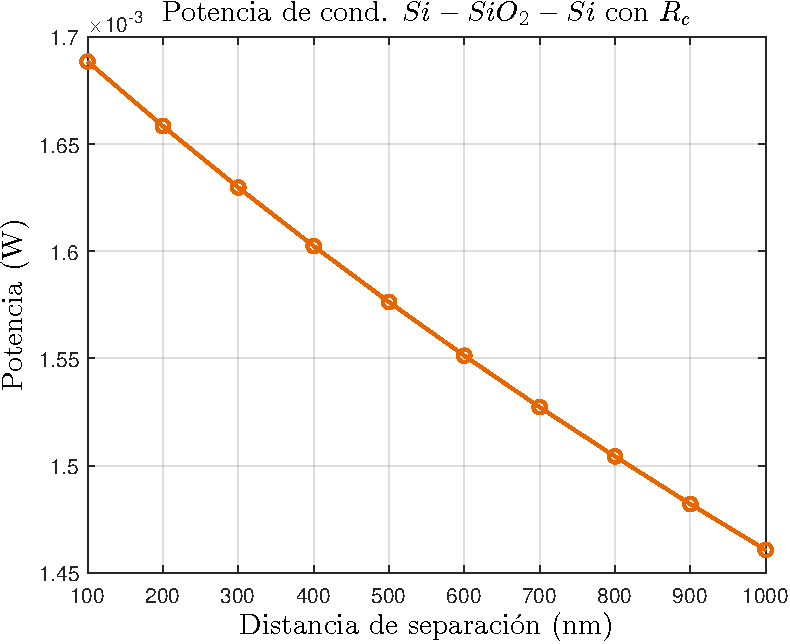
\includegraphics[width=1.0\textwidth]{figuras/Resultados/conduccion/pdf/Prc2_SiSiO2Si.pdf}
		\caption{Potencia solo con $R_c$}
		\label{fig:Prc2_SiSiO2Si}
	\end{subfigure}
	\caption[Efectos de la resistencia de contacto sobre el flujo de calor por conducción]{Representación gráfica del flujo de calor por conducción frente a las diferentes alturas del nano-espaciador con y sin $R_c$. (\subref{fig:Prc_SiSiO2Si}) Comparación de la potencia conducida de un nano-espaciador sin $R_c$ y con $R_c$ sobre un mismo eje.(\subref{fig:Prc2_SiSiO2Si})  Potencia conducida de un nano-espaciador con $R_c$.}
	\label{fig:PcondRc_SiSiO2Si}
\end{figure}
Para un área de 9$\mu m^2$ la resistencia de contacto total es aproximadamente de $444.44\cdot 10^3 \ K/W$ comparada con los $85.43\cdot 10^3 \ K/W$ de la mayor resistencia que presenta el nano-espaciador con 1000nm de altura a 25\textdegree C es al menos 5 veces más grande, por lo cual, como se observa en la figura \ref{fig:Prc_SiSiO2Si} la resistencia de contacto constante domina sobre la resistencia del nano-espaciador dando así la forma aproximada de una recta (figura \ref{fig:Prc2_SiSiO2Si}) porque la mayor caída de temperatura se dá en la superficie de contacto, evitando que aumente la temperatura del nano-espaciador variando menos su resistencia térmica (figuras \ref{fig:Pcond_SiSiO2Si_CFD} y \ref{fig:Pcond_SiSiO2Si_Rc_CFD}).
\graphicspath{ {./figuras/Resultados/conduccion/} }
\begin{figure}[H]
	\centering 		% cond sin Rc
	\begin{subfigure}[b]{0.49\textwidth}
	\centering
		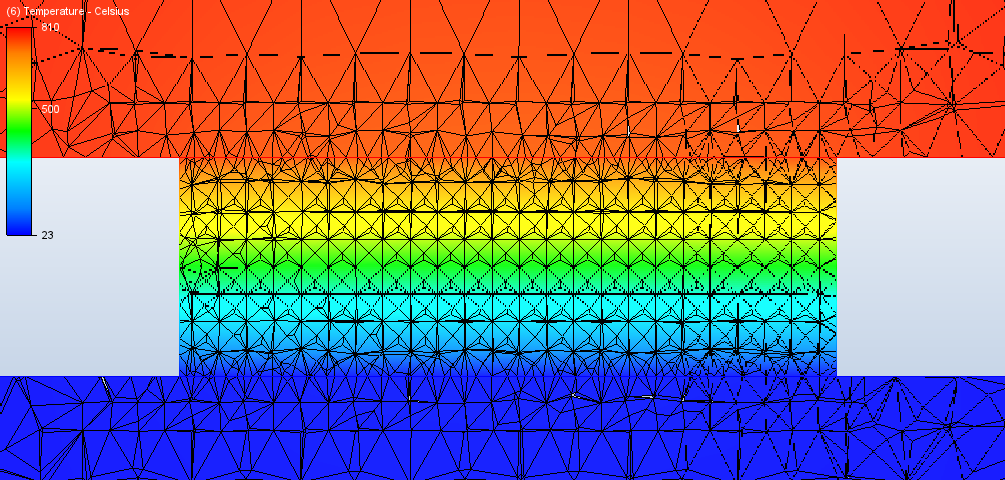
\includegraphics[width=1.00\textwidth]{SiSiO2Si_1000nm_Plane.png}
		\caption{sin $R_c$}
	\label{fig:Pcond_SiSiO2Si_CFD}
\end{subfigure}
\hfill 					% cond con Rc
\begin{subfigure}[b]{0.49\textwidth}
	\centering
		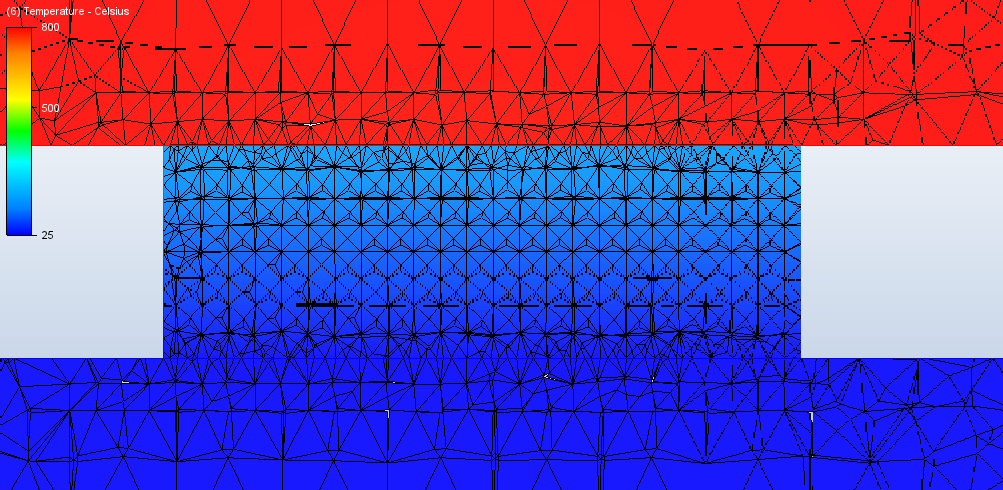
\includegraphics[width=1.00\textwidth]{SiSiO2Si_1000nm_Plane_Rc.png}
		\caption{con $R_c$}
	\label{fig:Pcond_SiSiO2Si_Rc_CFD}
\end{subfigure}
\caption{Resultados gráficos de la simulación de CFD de la transmisión de calor por conducción a través de un nano-espaciador de 1000nm de altura sin $R_c$ (\subref{fig:Pcond_SiSiO2Si_CFD}) y con $R_c$ (\subref{fig:Pcond_SiSiO2Si_Rc_CFD}).}
	\label{fig:Pconds_SiSiO2Si_CFD}
\end{figure}
La disminución de flujo de calor por conducción es significativa para todos los casos, siendo la potencia de conducción con $R_c$ variando aproximadamente entre un 3\% y un 14\% de la potencia sin $R_c$, lo que implica una disminución de conducción de unos 97\% y 85\%.\\\\
Hay que tomar en cuenta que la resistencia de contacto en la realidad no es constante con la temperatura a diferencia de las simulaciones en CFD donde la $R_c$ es constante, pero sirve para tener una primera idea de su importancia en la eliminación de la transferencia de calor por conducción.
\subsection{Efecto de la porosidad sobre la conducción}
\begin{figure}[H]
\centering
	\begin{subfigure}[b]{0.49\textwidth}
		\centering
		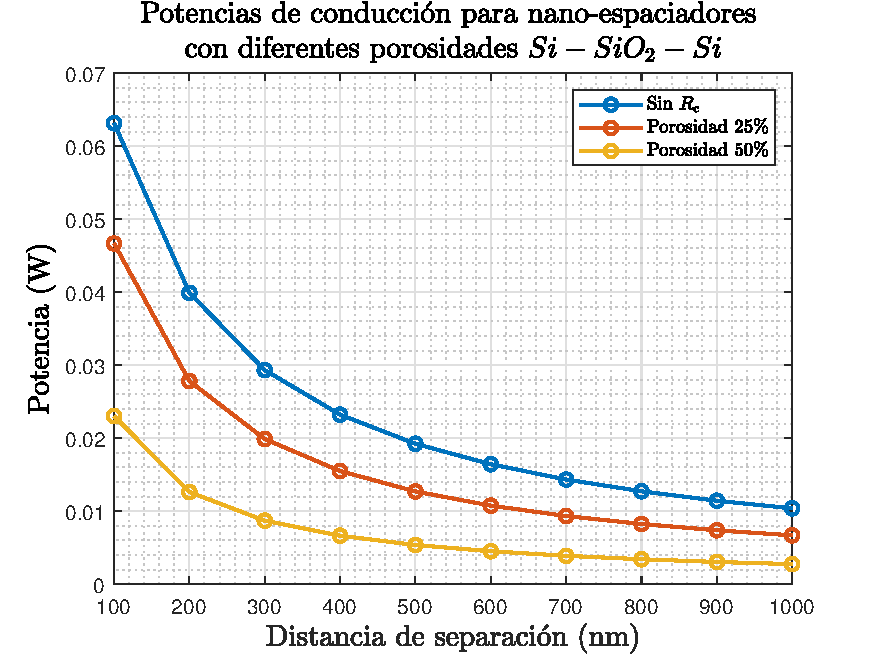
\includegraphics[width=1.0\textwidth]{figuras/Resultados/conduccion/pdf/Ppor_SiSiO2Si.pdf}
		\caption{Efecto de la Porosidad}
		\label{fig:Ppor_SiSiO2Si}
	\end{subfigure}
	\hfill
	\begin{subfigure}[b]{0.49\textwidth}
		\centering
		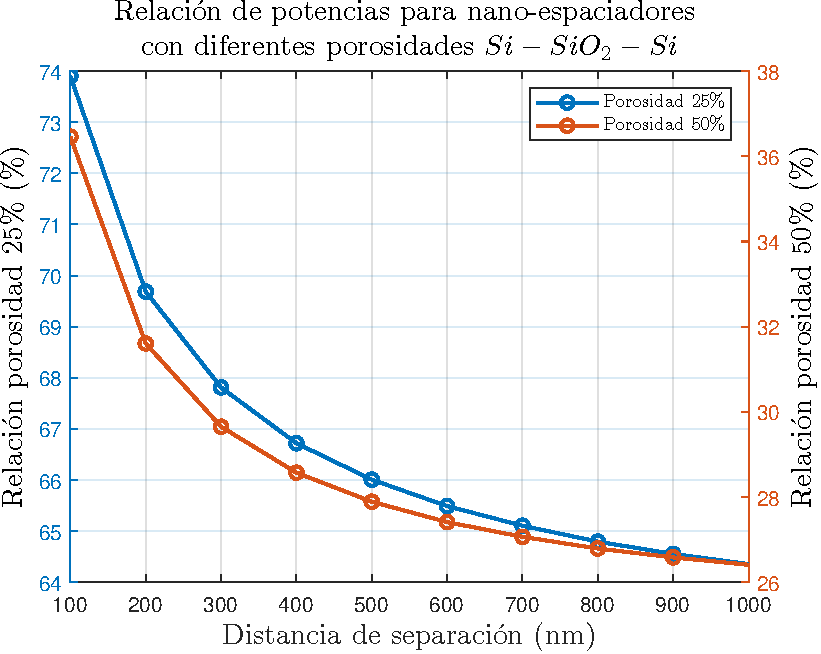
\includegraphics[width=1.0\textwidth]{figuras/Resultados/conduccion/pdf/relPpor_SiSiO2Si.pdf}
		\caption{Efecto de la Porosidad relativo}
		\label{fig:relPpor_SiSiO2Si}
	\end{subfigure}
	\caption[Efectos de la porosidad del nano-espaciador sobre el flujo de calor por conducción]{(\subref{fig:Ppor_SiSiO2Si}) Representación gráfica de las potencias de calor transmitidas por conducción  a través de un nano-espaciador frente a la variación de la altura del nano-espaciador para diferentes grados de porosidad del 0\%, 25\% y 50\% del $SiO_2$ y su modelo analítico (ec. \eqref{eq:Pcond_d_p}). (\subref{fig:relPpor_SiSiO2Si}) Representación gráfica de las relaciones de las potencias por conducción para porosidades del $SiO_2$ de 25\% y 50\% respecto a la potencia de 0\% de porosidad frente a la variación de la altura del nano-espaciador.}
	\label{fig:PcondPor_SiSiO2Si}
\end{figure}
%% Ahora a comentar sobre las porosidades
Para diferentes porosidades la conductividad térmica varía, disminuyendo con el aumento del grado de porosidad \cite{ThermalConductivity_SiO2_2018}, por este motivo la potencia de conducción disminuye para todas las alturas de nano-espaciador. La relación o conductividad térmica normalizada para una porosidad del 25\% y 50\% son respectivamente 0.64 y 0.25 veces la conductividad térmica del material \cite{ThermalConductivity_SiO2_2018}.\\\\
Como se puede observar en la figura \ref{fig:Prc2_SiSiO2Si} las relaciones de potencia no se cumplen completamente porque la temperatura en todo el nano-espaciador no es la misma lo que produce que la conductividad térmica a lo largo del espaciador sea distinta. Por tal motivo, al disminuir la altura del nano-espaciador aumenta la relación porque aumenta el gradiente de temperatura.\\\\
Utilizando la aplicación \textbf{Curve Fitting} de MATLAB se obtiene un modelo matemático que relaciona la potencia de conducción respecto a la altura del nano-espaciador ($d$) y la porosidad del material del nano-espaciador ($\rho$), como se muestra en la ecuación \eqref{eq:Pcond_d_p} donde $d$ es en nanómetros.
\begin{equation}
P(d,\rho)=- \frac{  16.47\cdot \rho-11.03 }{d-106.80\cdot \rho +74.68}
\label{eq:Pcond_d_p}
\end{equation}
%% RAD Si-SiO2-Si
\subsection{Radiación de campo cercano}
Para la radiación por campo cercano se utiliza la aplicación descrita en la sección \ref{sec:calc_campo_cercano} para dos placas gruesas de $Si$ para varias separaciones entre ellas. La potencia radiativa (figura \ref{fig:rad_SiSi_ds}) aumenta con la disminución de la distancia de separación como lo indica el componente exponencial en la ecuación \eqref{eq:flujoEvasNF} de \cite{nfTPV_equations}.
\begin{figure}[H]
	\centering
		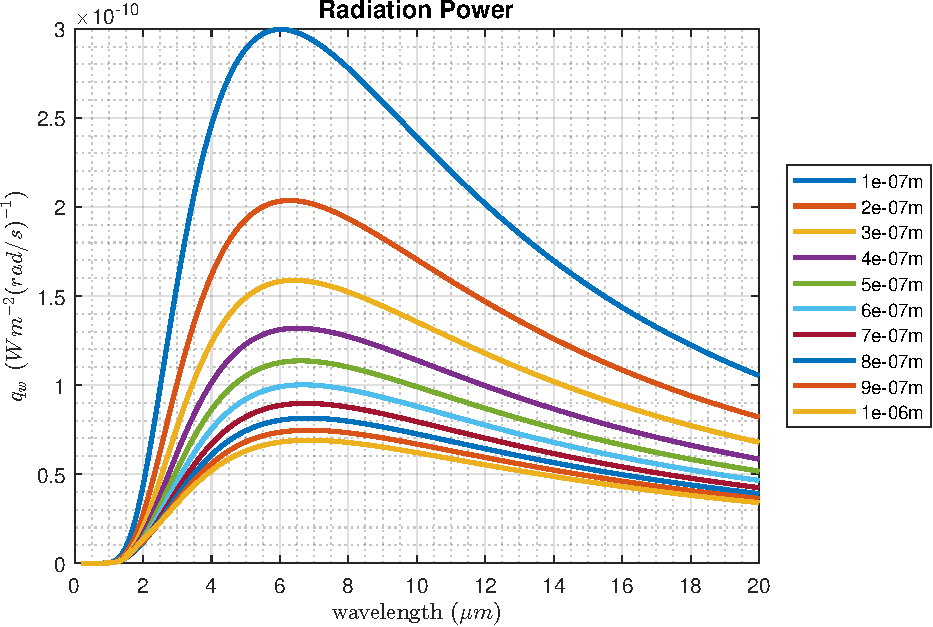
\includegraphics[width=0.7\textwidth]{figuras/Resultados/radiacion/SiSi_ds.pdf}
	\caption{Potencia de radiación monocromática para dos placas gruesas planas de $Si$ en todo el rango espectral frente a diferentes distancias de separación de las placas ($d$) en metros.}
	\label{fig:rad_SiSi_ds}
\end{figure}
Integrando la potencia en el rango espectral de longitudes de onda con energías mayores a 1.1 eV, energía de banda del $Si$, se obtiene en promedio potencias del orden de $60 \ W/m^2$ (figura \ref{fig:prad_Eg11_SiSi}) a diferencia de integrar en todo el rango espectral, hasta las $\sim$20 $\mu m$, cuyo orden es de $10^4 \ W/m^2$ (figura \ref{fig:prad_full_SiSi}), Lo cual indica que se desaprovecha una gran cantidad de energía.
\begin{figure}[H]
	\centering
		\begin{subfigure}[b]{0.49\textwidth}
	\centering
		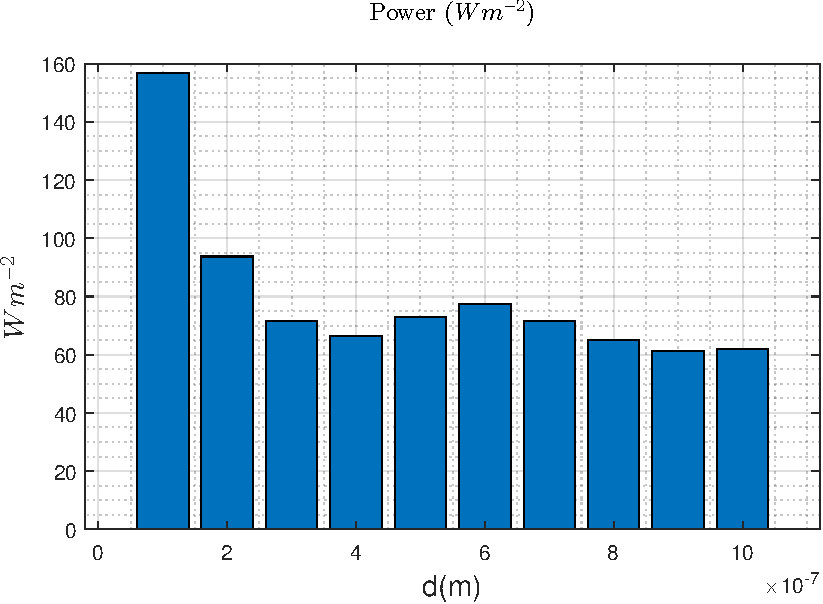
\includegraphics[width=1.00\textwidth]{figuras/Resultados/radiacion/p_11_SiSi.pdf}
	\caption{Potencia para energía mayor a 1.1 eV}
	\label{fig:prad_Eg11_SiSi}
\end{subfigure}
\hfill
\begin{subfigure}[b]{0.49\textwidth}
	\centering
		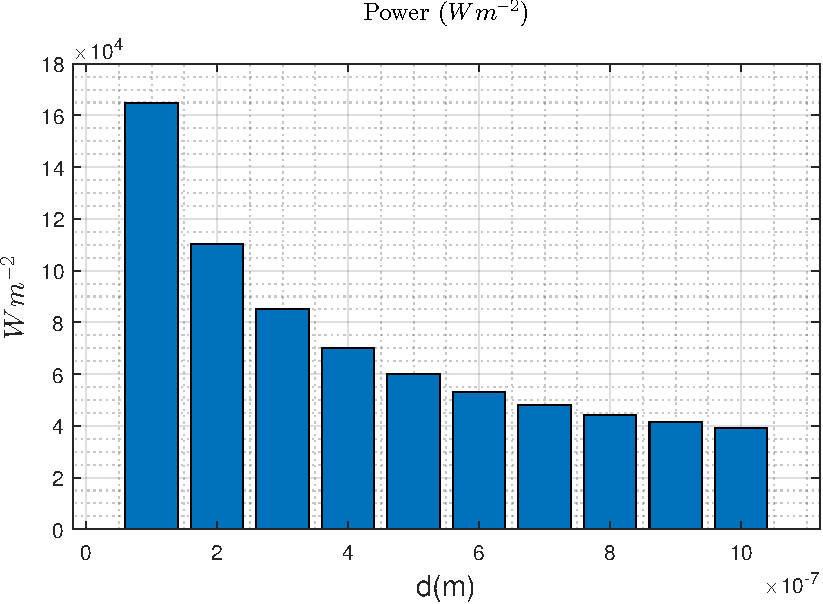
\includegraphics[width=1.00\textwidth]{figuras/Resultados/radiacion/p_full_SiSi.pdf}
	\caption{Potencia hasta las $\sim$20 $\mu m$}
	\label{fig:prad_full_SiSi}
\end{subfigure}
	\caption{Potencias por unidad de área transmitida por radiación por efecto de campo cercano para el rango espectral de energía mayor a 1.1 eV (\subref{fig:prad_Eg11_SiSi}) y para todo el rango espectral (\subref{fig:prad_full_SiSi}) frente a las diferentes distancias de separación.}
	\label{fig:prad_SiSi}
\end{figure}
Las potencias radiadas obtenidas para el rango de longitudes de onda mayor a la banda energética del $Si$ son muy pequeñas (figura \ref{fig:prad_Eg11_SiSi}), produciendo que no sea viable este sistema porque las pérdidas por conducción son demasiado grandes. Esto se puede visualizar en la figura \ref{fig:rel_SiSi11_Rc}, donde ni siquiera asumiendo la presencia de un único nano-espaciador con Rc se consigue que la potencia radiada sea al menos un orden de magnitud más alta que la potencia transferida por conducción (no se alcanza un factor 10).
\begin{figure}[H]
	\centering
\begin{subfigure}[b]{0.49\textwidth}
	\centering
		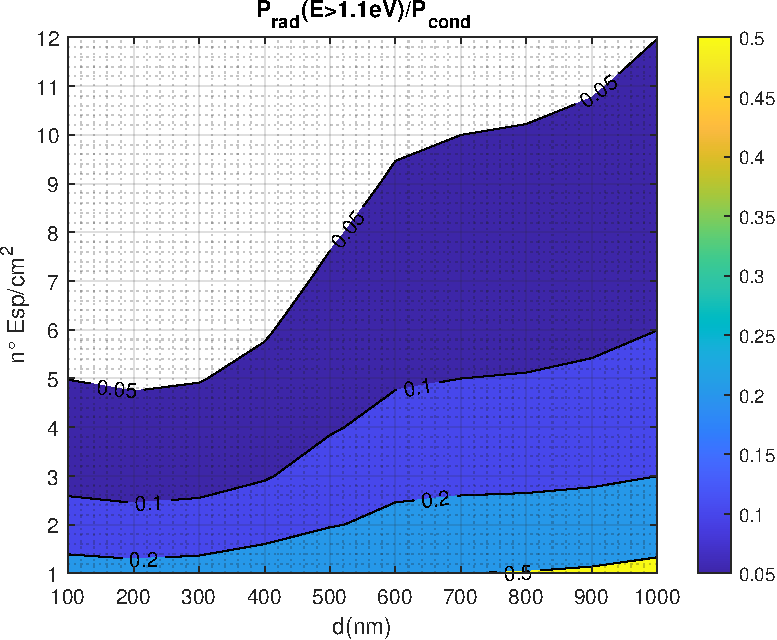
\includegraphics[width=1.00\textwidth]{figuras/Resultados/RelacionCondRad/rel_SiSi11.pdf}
	\caption{Relación de potencias para Eg$>$1.1 eV}
	\label{fig:rel_SiSi11}
\end{subfigure}
\hfill
\begin{subfigure}[b]{0.49\textwidth}
	\centering
		\includegraphics[width=1.00\textwidth]{figuras/Resultados/RelacionCondRad/rel_SiSi11_Rc.pdf}
	\caption{Relación de potencias para Eg$>$1.1 eV con $R_c$}
	\label{fig:rel_SiSi11_Rc}
\end{subfigure}
\caption{Densidad de los nano-espaciadores para diferentes relaciones de las potencias de radiación en el rango espectral de energía mayor a 1.1 eV respecto a las de conducción para cada densidad de nano-espaciadores de un sistema nTPV de 1$cm^2$ y célula de $Si$ sin $R_c$ (\subref{fig:rel_SiSi11}) y con $R_c$ (\subref{fig:rel_SiSi11_Rc}) frente a las diferentes alturas de los nano-espaciadores. La barra de colores al lateral de cada gráfica representa todas las relaciones entre ambas potencias para diferentes densidades de nano-espaciadores en el rango que se muestra en los extremos de cada barra. También se muestran los contornos con su valor para destacar las distintas relaciones existentes de una manera sencilla.}
	\label{fig:rels_SiSi11}
\end{figure}
%% RELACION ENTRE COND Y RAD
Para tener una primera mejor idea de los valores numéricos de los resultados obtenidos de las simulaciones de transmisión de calor por conducción y radiación de campo cercano se recolectan en la tabla \ref{tab:condTerSiSiO2Si}, estando en notación científica y con los decimales necesarios para una clara diferenciación de los resultados con el cambio de la distancia de separación entre emisor y célula.
\begin{table}[H]
	\centering
		\begin{tabular}{|c||c|c|c|c||c|c|}
		\hline
			\multirow{2}{*}{ }& \multicolumn{6}{c|}{\textbf{\large Potencias según como se transmite el calor}}\\ \cline{2-7}
		  & \multicolumn{4}{c||}{Conducción (W/nº nano-espaciadores)}& \multicolumn{2}{c|}{Radiación $(W/m^2)$}\\ \hline
			Dist. (nm)&$P_{Normal}$&$P_{R_c-Empirico}$&$P_{Porosidad25}$&$P_{Porosidad50}$&$P_{Eg>1.1eV}$&$P_{full}$\\ \hline \hline
			100&6,31E-02&1,69E-03&4,67E-02&2,30E-02&156.89&1,65E+05\\ \hline
			200&3,99E-02&1,66E-03&2,78E-02&1,26E-02&93.75&1,10E+05\\ \hline
			300&2,93E-02&1,63E-03&1,99E-02&8,69E-03&71.75&8,51E+04\\ \hline
			400&2,32E-02&1,60E-03&1,55E-02&6,63E-03&66.39&7,01E+04\\ \hline
			500&1,92E-02&1,58E-03&1,27E-02&5,36E-03&73.00&6,02E+04\\ \hline
			600&1,64E-02&1,55E-03&1,08E-02&4,50E-03&77.52&5,32E+04\\ \hline
			700&1,43E-02&1,53E-03&9,33E-03&3,88E-03&71.63&4,80E+04\\ \hline
			800&1,27E-02&1,50E-03&8,24E-03&3,41E-03&64.90&4,43E+04\\ \hline
			900&1,14E-02&1,48E-03&7,38E-03&3,04E-03&61.42&4,14E+04\\ \hline
		 1000&1,04E-02&1,46E-03&6,68E-03&2,74E-03&62.09&3,93E+04\\ \hline
		\end{tabular}
	\caption{Tabla de resultados de las simulaciones de conducción y radiación de campo cercano para diferentes alturas del nano-espaciador. Flujos de calor del nTPV $Si-SiO_2-Si$ para diferentes alturas del nano-espaciador, para los casos sin $R_c$ y con $R_c$ igual a $4 \cdot 10^{-6} \ m^2 K/W$ \cite{nf_TPV_Pillars_SiO2}, y sin $R_c$ pero con las proporciones de las porosidades de \cite{ThermalConductivity_SiO2_2018} para un 25\% y un 50\%.}
	\label{tab:condTerSiSiO2Si}
\end{table}
\vfill \newpage
%%% AHORA EL CASO DE Si SiO2 y Ge
\section{Resultados de las simulaciones para una nTPV de Si-SiO2-Ge}
A continuación se procede a estudiar un caso más realista del sistema nTPV descrito en la sección anterior con una célula de $Ge$ en vez de una de $Si$, cuya banda energética es de 0.7 eV respecto a los 1.1 eV del $Si$.
\subsection{Simulaciones de CFD}
Se realizan las simulaciones de transmisión de calor por conducción en CFD, obteniéndose una reducción considerable de la potencia de la nTPV con $R_c$ (figura \ref{fig:Prc_SiSiO2Ge}) respecto a sin $R_c$ (figura \ref{fig:Pn_SiSiO2Ge}), como en el caso de la célula de $Si$ (figuras \ref{fig:PcondRc_SiSiO2Si} \subref{fig:Prc_SiSiO2Si} y \subref{fig:Prc2_SiSiO2Si}).
\graphicspath{ {./figuras/Resultados/conduccion/pdf/} }
\begin{figure}[H]
	\centering
	%% Si-SiO2-Si Eg
	\begin{subfigure}[b]{0.49\textwidth}
		\centering
		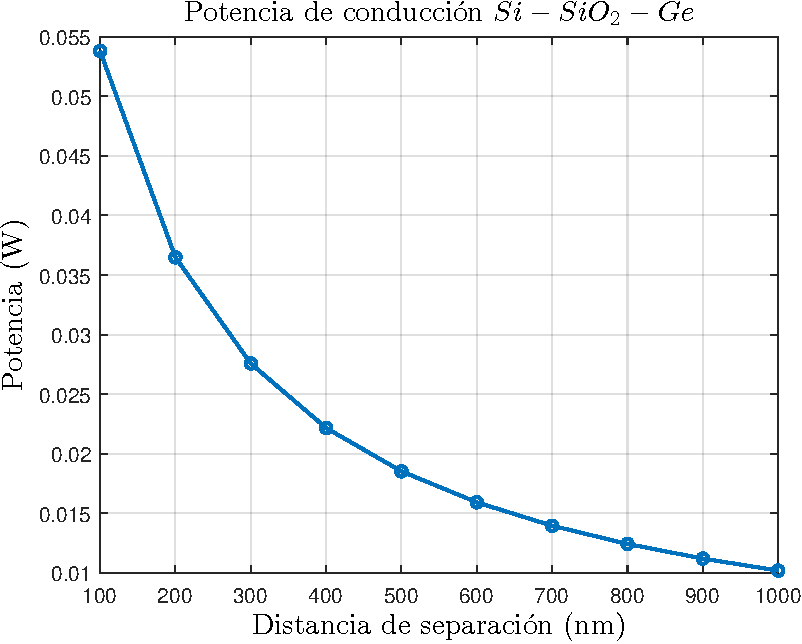
\includegraphics[width=1\textwidth]{Pn_SiSiO2Ge.pdf}
		\caption{Potencia cond. sin $R_c$}
		\label{fig:Pn_SiSiO2Ge}
	\end{subfigure}
	\hfill
	\begin{subfigure}[b]{0.49\textwidth}
		\centering
		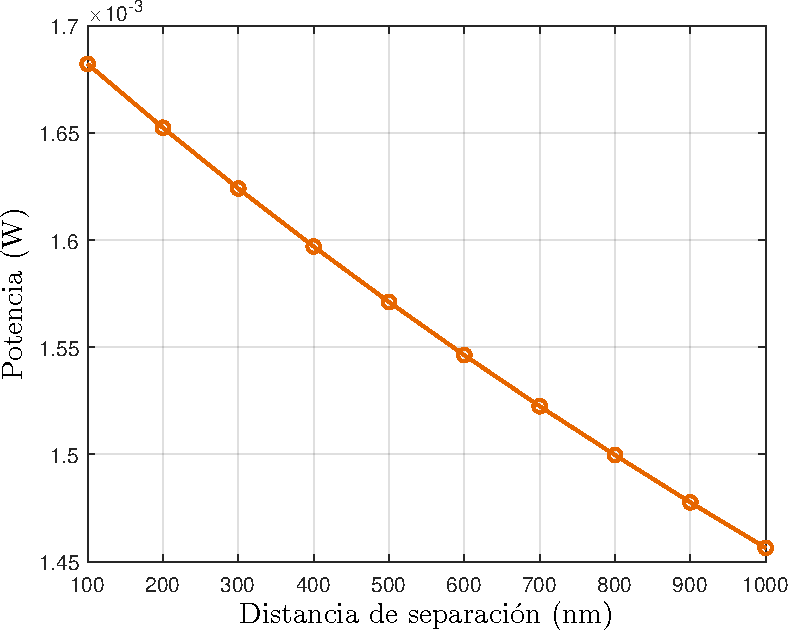
\includegraphics[width=1.00\textwidth]{Prc2_SiSiO2Ge.pdf}
		\caption{Potencia cond. con $R_c$}
		\label{fig:Prc_SiSiO2Ge}
	\end{subfigure}
	\caption{Potencias de conducción para un sistema nTPV de $Si-SiO_2-Ge$ de un nano-espaciador con emisor a 800\textdegree C y célula a 25\textdegree C sin $R_c$ (\subref{fig:Pn_SiSiO2Ge}) y con $R_c$ (\subref{fig:Prc_SiSiO2Ge}) frente a las diferentes alturas del nano-espaciador.}
	\label{fig:Pcond_SiSiO2Ge}
\end{figure}
La potencia de conducción con $R_c$ disminuye de unos 53.80 $mW$ sin $R_c$ a unos 1.68 $mW$ para una altura de nano-espaciador de 100nm, que representa una relación del 3.13\%. Para unos 1000nm de altura de nano-espaciador la potencia disminuye de unos 10.20 $mW$ sin $R_c$ a unos 1.46 $mW$ con $R_c$, que representa una relación del 14.31\%.\\\\
Comparando los resultados obtenidos de la simulación de transmisión de calor por conducción de la nTPV de célula de $Ge$ respecto a la de $Si$, ambas con $R_c$, se obtiene una relación mayor del 99\% para todas las alturas del nano-espaciador, dando a entender que la diferencia de la conductividad térmica de los materiales no produce un efecto significativo sobre la conducción con la existencia de $R_c$, a diferencia de la nTPV sin $R_c$ donde la relación varía entre un $\sim$85\% y un $\sim$98\%.
\vfill
\subsection{Radiación de campo cercano}
De las simulaciones de radiación de campo cercano se obtienen también resultados muy parecidos a los obtenidos en el caso de la célula de $Si$ (figura \ref{fig:SiSi_vs_SiGe}), solo mostrándose hasta los $\sim$14$\mu m$ de longitud de onda, donde se observa como al disminuir la distancia de separación aumenta la potencia radiativa (figura \ref{fig:rad_SiGe}).
\begin{figure}[H]
\centering
\begin{subfigure}[b]{0.49\textwidth}
	\centering
		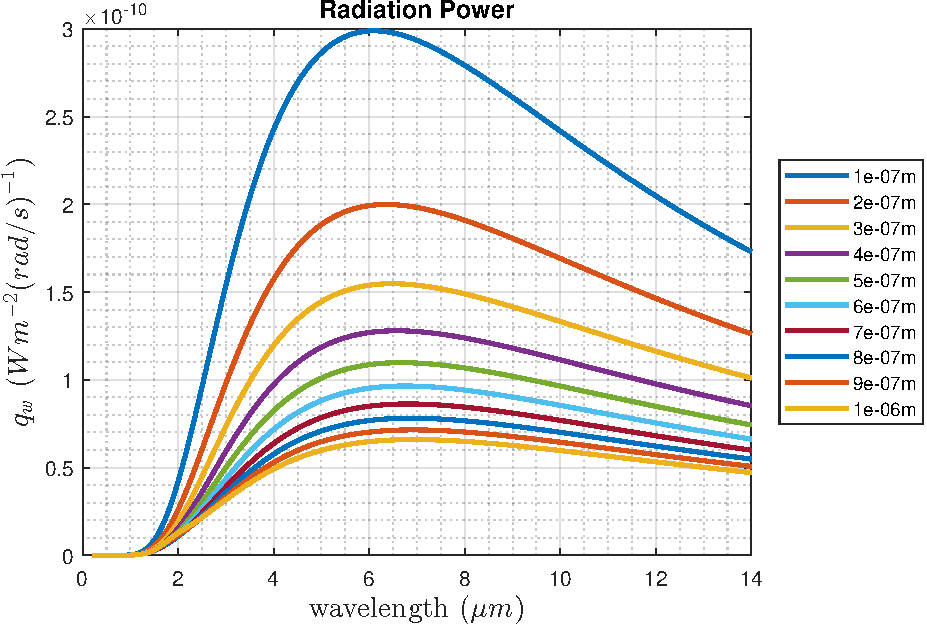
\includegraphics[width=1.00\textwidth]{figuras/Resultados/radiacion/SiGe.pdf}
	\caption{Potencia monocromática para varias $d$}
	\label{fig:rad_SiGe}
\end{subfigure}
\hfill
\begin{subfigure}[b]{0.49\textwidth}
	\centering
		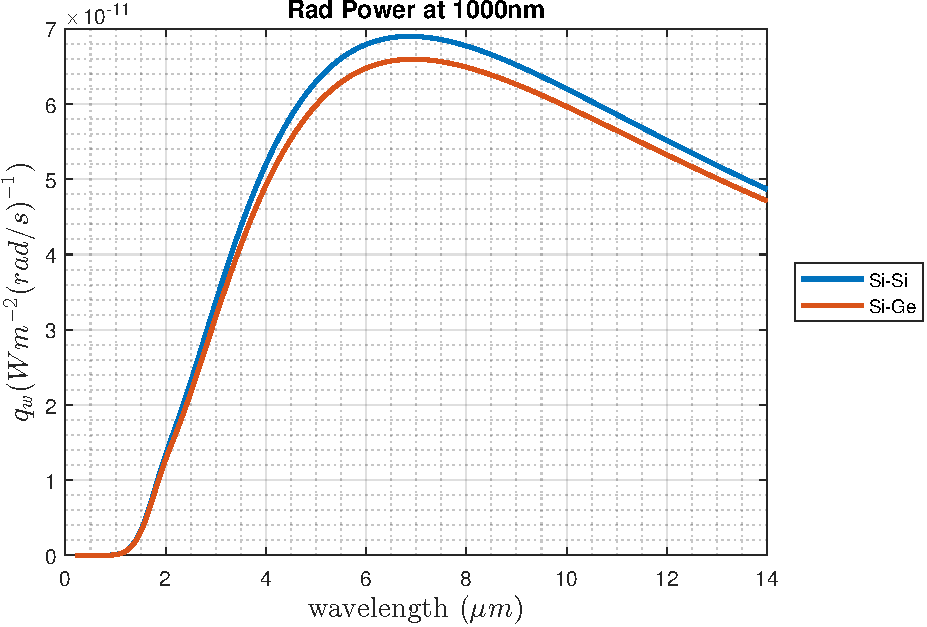
\includegraphics[width=1.00\textwidth]{figuras/Resultados/radiacion/SiSi_vs_SiGe.pdf}
	\caption{Comparación de células de $Si$ y $Ge$}
	\label{fig:SiSi_vs_SiGe}
\end{subfigure}
\caption{Potencias de radiación monocromática por campo cercano para un sistema nTPV $Si-SiO_2-Ge$ frente a las longitudes de onda para varias distancias de separación entre placas(\subref{fig:rad_SiGe}) y para dos materiales de célula, $Si$ y $Ge$ (\subref{fig:SiSi_vs_SiGe}).}
\label{fig:rads_SiGe}
\end{figure}
Para la obtención de las potencias de radiación se procede a realizar la integral en el rango espectral de energía mayor a los 0.7 eV, obteniéndose potencias alrededor de los $10^3 \ W/m^2$ (figura \ref{fig:p_Eg_SiGe}), y para todo el rango espectral de longitudes de onda se obtiene potencias alrededor de los $10^4 \ W/m^2$ con un máximo de $\sim$1.5$10^5 \ W/m^2$ (figura \ref{fig:p_full_SiGe} y tabla \ref{tab:SiSiO2Ge}). 
%% POTENCIAS INTEGRADAS
\begin{figure}[H]
\centering
\begin{subfigure}[b]{0.49\textwidth}
	\centering
		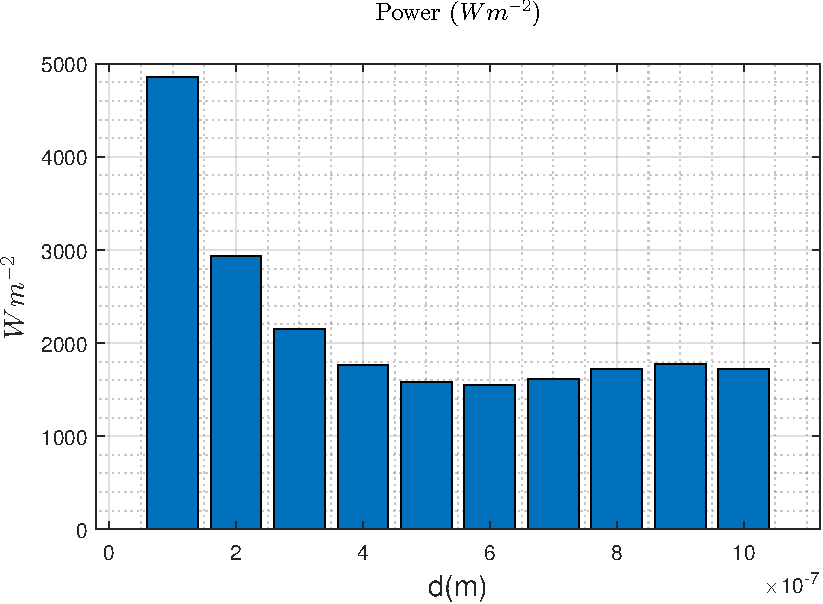
\includegraphics[width=1.00\textwidth]{figuras/Resultados/radiacion/p_Eg_SiGe.pdf}
	\caption{Potencia para Eg$>$0.7eV}
	\label{fig:p_Eg_SiGe}
\end{subfigure}
\hfill
\begin{subfigure}[b]{0.49\textwidth}
	\centering
		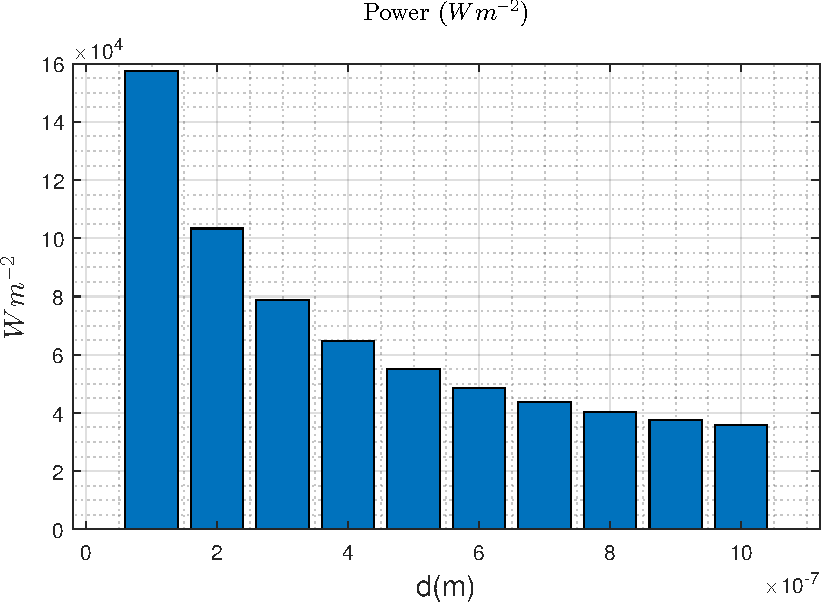
\includegraphics[width=1.00\textwidth]{figuras/Resultados/radiacion/p_full_SiGe.pdf}
	\caption{Potencia hasta $\sim$14$\mu m$}
	\label{fig:p_full_SiGe}
\end{subfigure}
	\caption[Potencias por unidad de área para la radiación de campo cercano para el sistema $Si-SiO_2-Ge$ frente a las diferentes alturas del nano-espaciador]{Potencias por unidad de área para la radiación de campo cercano para el sistema $Si-SiO_2-Ge$ frente a las diferentes alturas del nano-espaciador. (\subref{fig:p_Eg_SiGe}) Potencias en el rango espectral de todas las longitudes de onda de energía mayor a 0.7 eV. (\subref{fig:p_full_SiGe}) Potencias en todo el rango espectral, hasta las $\sim$14$\mu m$.}
	\label{fig:p_SiGe}
\end{figure}
Como para el caso de la nTPV de $Si-SiO_2-Si$ la diferencia de la potencia entre integrar hasta los 0.7 eV del rango espectral e integrar en todo el rango espectral es significativa. Al cambiar la célula de $Si$ por una de menor energía de banda de $Ge$ se aumenta la cantidad de potencia que se puede convertir en electricidad. También se observa una disminución de las potencias alrededor de los 600nm (figura \ref{fig:p_Eg_SiGe}), a diferencia de la célula de $Si$ que aumenta (\ref{fig:prad_Eg11_SiSi}).
%%%   DENSIDAD DE NANO-ESPACIADORES
\subsection{Densidad de nano-espaciadores}
Para tener una mejor percepción de las ventajas que presenta el usar una célula de $Ge$ frente a una de $Si$ se calcula la densidad de nano-espaciadores frente a las alturas del nano-espaciador para todas las relaciones de la potencia de radiación respecto a la de conducción mayores que 3 o 10.\\\\
Hay que tener en cuenta que para un centímetro cuadrado de superficie de radiación la transmisión de calor por radiación se ve multiplicado por $10^{-4}$, por lo tanto, la potencia de radiación con $E_g>0.7eV$ en un centímetro cuadrado es $\sim$10 mayor que la potencia conducida sin resistencia de contacto para un nano-espaciador (figura \ref{fig:rel_SiSiO2Ge}), pero $\sim$100 veces mayor que la potencia conducida con resistencia de contacto (figura \ref{fig:rel_SiSiO2Ge_Rc}).
\begin{figure}[H]
	\centering
	%% Si-SiO2-Si Eg
	\begin{subfigure}[b]{0.49\textwidth}
		\centering
		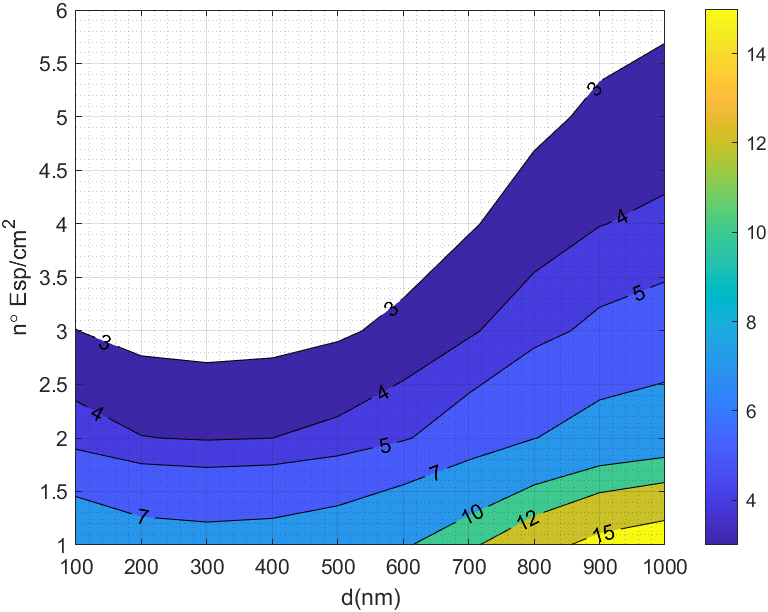
\includegraphics[width=1.00\textwidth]{figuras/Resultados/RelacionCondRad/SiGe.png}
		\caption{$E>0.7eV$, sin $R_c$}
		\label{fig:rel_SiSiO2Ge}
	\end{subfigure}
	\hfill
	\begin{subfigure}[b]{0.49\textwidth}
			\centering
			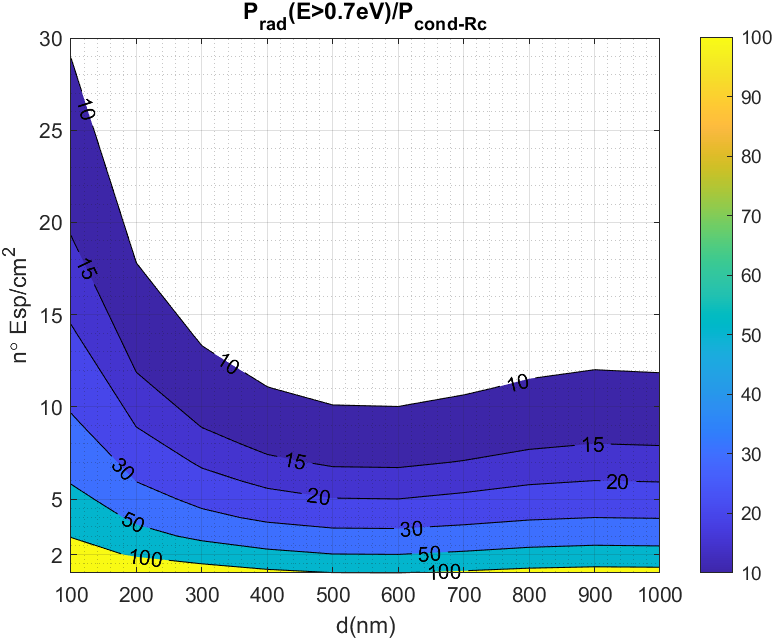
\includegraphics[width=1.00\textwidth]{figuras/Resultados/RelacionCondRad/SiGe_Rc.png}
			\caption{$E>0.7eV$, con $R_c$}
			\label{fig:rel_SiSiO2Ge_Rc}
		\end{subfigure}
	\caption{Densidad de nano-espaciadores por $cm^2$ frente a las alturas de los nano-espaciadores para todas las relaciones de la potencia de radiación en el rango espectral de energías mayores e igual a 0.7 eV respecto a las potencias de conducción (dependencia en la densidad de nano-espaciadores) mayores a 3 para el caso sin $R_c$ (\subref{fig:rel_SiSiO2Ge}) y mayores a 10 para el caso con $R_c$ (\subref{fig:rel_SiSiO2Ge_Rc}). Donde las barras de colores laterales representan los colores asociados a cada uno de los valores de las relaciones de las potencias, con los contornos de las relaciones más significativas en los gráficos.}
	\label{fig:relation_SiSiO2Ge}
\end{figure}
Como se observa en las figuras \ref{fig:relation_SiSiO2Ge} \subref{fig:rel_SiSiO2Ge} y \subref{fig:rel_SiSiO2Ge_Rc}, la forma de la curva cambia su tendencia según se incluya o no la $R_c$ porque sin $R_c$ la tendencia de la curva de crecer con el aumento de la altura de los nano-espaciadores está marcada por la potencia de conducción (inversamente proporcional), y para el caso con $R_c$ la  tendencia de la curva de aumentar con la disminución de la altura de los nano-espaciadores está marcada por la potencia de radiación de campo cercano.\\\\
Los valores de las relaciones entre ambas potencias no son muy altos para el caso sin $R_c$, apenás consiguiendo seguro un factor de relación de al menos un orden de magnitud solo para una altura de un nano-espaciador de al menos unos 600nm, a diferencia del caso con $R_c$ que se consigue como mínimo una relación de dos ordenes de magnitud para todas las alturas de un nano-espaciador. Estas relaciones disminuyen con el aumento de la densidad de los nano-espaciadores porque aumenta la potencia de conducción, por este motivo solo serán viables aquellas configuraciones que como mínimo tengan una relación de potencias de un orden de magnitud para una configuración mínima de cuatro nano-espaciadores.\\\\
Para la densidad de nano-espaciadores se nota en la figura \ref{fig:rel_SiSiO2Ge_Rc} que el valor máximo para una relación de potencias de un orden de magnitud es aproximadamente 30, que es aproximadamente 10 veces respecto a la del caso sin $R_c$ (menor que 3) para la misma altura de nano-espaciadores (figura \ref{fig:rel_SiSiO2Ge}), y el valor para la misma relación de potencias para una altura de nano-espaciadores de 1000nm es 12, que es entre 6 y 12 veces respecto al caso sin $R_c$.\\\\
Por lo tanto, entre ambos casos el que puede ser viable es el sistema nTPV con $R_c$ porque presenta una mayor densidad de nano-espaciadores para una misma relación de potencias, lo que permite que se distribuya la carga sobre los nano-espaciadores y sea más fácil mantener la separación entre el emisor y la célula constante sobre toda la superficie.
\begin{figure}[H]
		\begin{subfigure}[b]{0.49\textwidth}
		\centering
		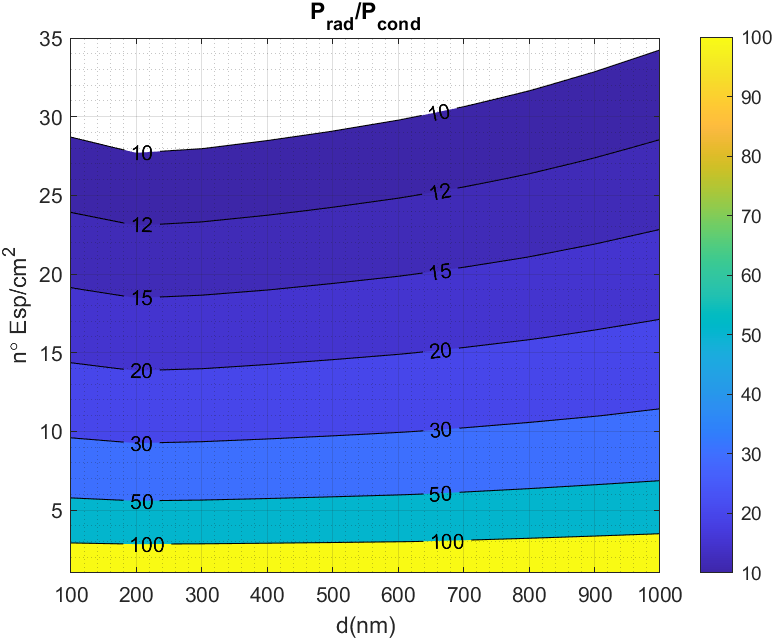
\includegraphics[width=1.00\textwidth]{figuras/Resultados/RelacionCondRad/SiGe_full.png}
		\caption{rango completo, sin $R_c$}
		\label{fig:rel_SiSiO2Ge_full}
	\end{subfigure}
		\hfill
		\begin{subfigure}[b]{0.49\textwidth}
			\centering
			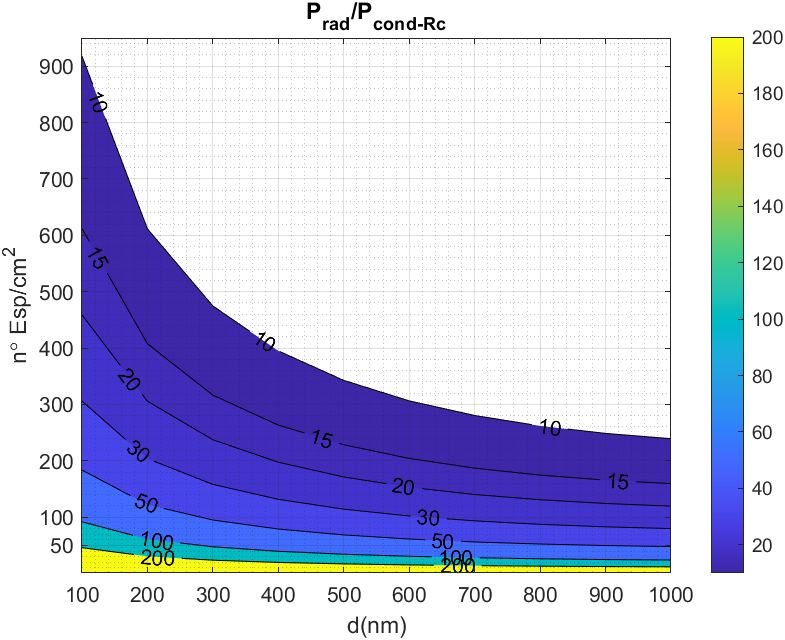
\includegraphics[width=1.00\textwidth]{figuras/Resultados/RelacionCondRad/SiGe_Rc_full_10.png}
			\caption{rango completo, con $R_c$}
			\label{fig:rel_SiSiO2Ge_Rc_full}
		\end{subfigure}
	\caption{Densidad de nano-espaciadores por $cm^2$ frente a las alturas de los nano-espaciadores para todas las relaciones de la potencia de radiación en todo el rango espectral respecto a las potencias de conducción (dependencia en la densidad de nano-espaciadores) mayores a 10 para el caso sin $R_c$ (\subref{fig:rel_SiSiO2Ge_full}) y para el caso con $R_c$ (\subref{fig:rel_SiSiO2Ge_Rc_full}). Donde las barras de colores laterales representan los colores asociados a cada uno de los valores de las relaciones de las potencias, con los contornos de las relaciones más significativas en los gráficos.}%
	\label{fig:rels_SiSiO2Ge_full}%
\end{figure}
Por último, se representan el caso de la densidad de nano-espaciadores frente a las alturas de los nano-espaciadores para varias relaciones de las potencias de radiación en todo el rango espectral y las potencias de conducción sin y con $R_c$ (figuras \ref{fig:rels_SiSiO2Ge_full}  \subref{fig:rel_SiSiO2Ge_full} y \subref{fig:rel_SiSiO2Ge_Rc_full}, respectivamente), observándose las mismas tendencias que para el rango espectral de energías mayores e iguales a 0.7 eV pero con mayor densidad de nano-espaciadores por el aumento de la potencia radiada de campo cercano.\\\\
Para facilitar la revisión de los resultados obtenidos de las simulaciones y de los cálculos realizados se agrupan en la tabla \ref{tab:SiSiO2Ge}, donde se presentan en notación científica para facilitar la observación de los ordenes de magnitud de los resultados.
\begin{table}[H]
	\centering
		\begin{tabular}{|c||c|c||c|c|}
		\hline
\multirow{2}{*}{ }& \multicolumn{4}{c|}{\textbf{\large Potencias según transmisión del calor}}\\ \cline{2-5}
& \multicolumn{2}{c||}{Conducción (W/nº esp.)}& \multicolumn{2}{c|}{Radiación $(W/m^2)$}\\ \hline
Dist. (nm)&$P_{Normal}$&$P_{R_c-Empirico}$&$P_{Eg>0.7eV}$&$P_{full}$\\ \hline \hline
100&5,38E-02&1,68E-03&4,87E+03&1,54E+05\\ \hline 
200&3,65E-02&1,65E-03&2,94E+03&1,01E+05\\ \hline 
300&2,76E-02&1,62E-03&2,16E+03&7,71E+04\\ \hline 
400&2,22E-02&1,60E-03&1,77E+03&6,31E+04\\ \hline 
500&1,85E-02&1,57E-03&1,59E+03&5,38E+04\\ \hline 
600&1,59E-02&1,55E-03&1,55E+03&4,74E+04\\ \hline 
700&1,39E-02&1,52E-03&1,62E+03&4,27E+04\\ \hline 
800&1,24E-02&1,50E-03&1,73E+03&3,93E+04\\ \hline 
900&1,12E-02&1,48E-03&1,78E+03&3,67E+04\\ \hline 
1000&1,02E-02&1,46E-03&1,73E+03&3,49E+04\\ \hline 
		\end{tabular}
	\caption{Tabla de las potencias de resultado de las simulaciones de transmisión de calor por radiación de campo cercano y conducción para el sistema nTPV $Si-SiO_2-Ge$.}
	\label{tab:SiSiO2Ge}
\end{table}
\vfill
%%% RESULTADOS DE SS
\section{Resultados de las simulaciones para una nTPV de SS-SiO2-Ge}
Un caso importante a estudiar es cuando el emisor es de acero inoxidable ($SS$) para la recuperación de calor residual porque en la industria se utiliza mucho el acero inoxidable como material para calderas, tuberías, entre otros componentes o máquinas que alcanzan altas temperaturas y que tienen que se enfriadas mediante un intercambiadores de calor que se conectan a turbinas de vapor para recuperar parte de la energía, presentando el problema de trabajar con fluidos y partes móviles que necesitan mantenimiento.\\\\
Para las simulaciones de transmisión de calor por conducción se estudian los efectos de resistencias de contacto aún mayores, obtenidas las conductancias de contacto entre dos trozos de acero 304 y mediante las ecuaciones \eqref{eq:relacion_conductividadesTermicas} y \eqref{eq:relacion_Rc} se obtienen las resistencia de contacto para una presión de $\sim$1 GPa por ser un valor con menor error respecto al modelo matemático \cite{experimental_Rc_SS}, siendo dicho valor aproximadamente unos 1000 $W/(m^2 K)$ .\\\\
La nueva resistencia de contacto calculada es $5.5\cdot 10^{-3} \ m^2 K/W$ y se toma un valor intermedio entre dicha resistencia de contacto y la resistencia de contacto empírica de $4\cdot 10^{-6} \ m^2 K/W$ \cite{nf_TPV_Pillars_SiO2} para obtener en mayor detalle los efectos de la resistencia de contacto sobre el flujo de calor por conducción, siendo el valor de dicha resistencia de contacto calculada intermedia unos $\sim 2.75\cdot 10^{-3} \ m^2 K/W$.
\begin{figure}[H]
	\centering
	\begin{subfigure}[b]{0.49\textwidth}
		\centering
			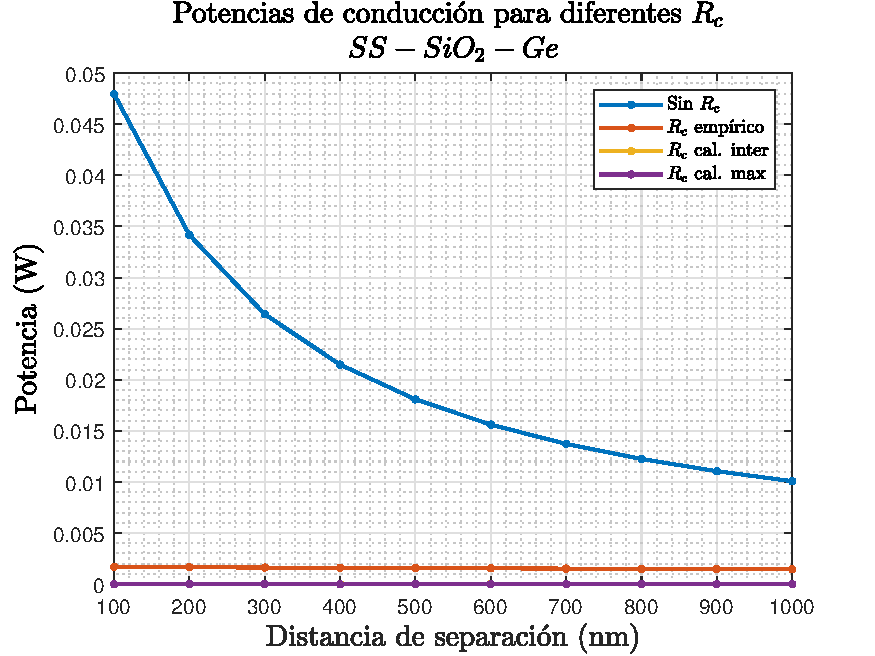
\includegraphics[width=1.00\textwidth]{figuras/Resultados/conduccion/pdf/Prcs_SsSiO2Ge.pdf}
		\caption{Potencias de conducción}
		\label{fig:Prcs_SsSiO2Ge}
	\end{subfigure}
	\hfill
	\begin{subfigure}[b]{0.49\textwidth}
		\centering
			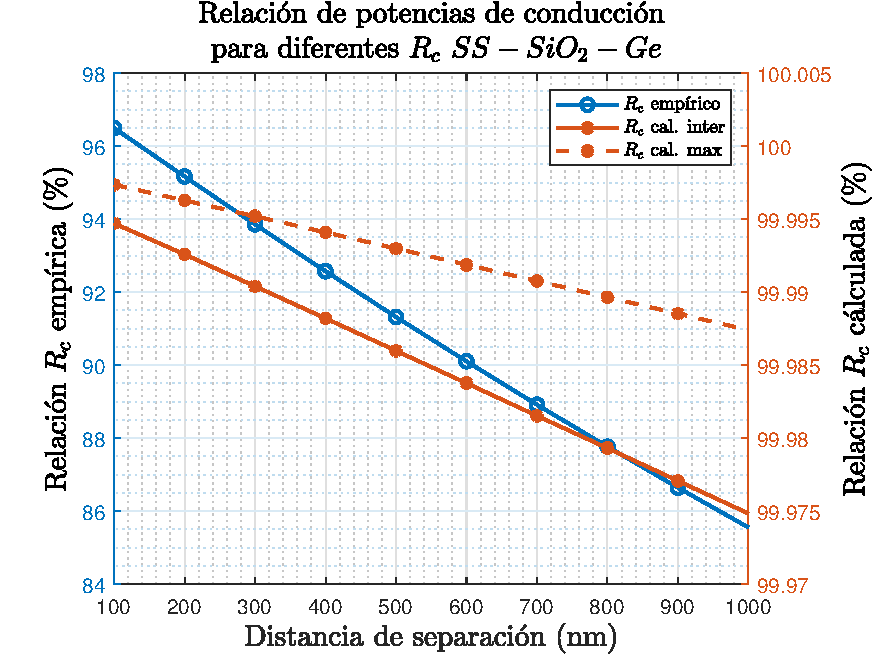
\includegraphics[width=1.00\textwidth]{figuras/Resultados/conduccion/pdf/relPrcs_SsSiO2Ge.pdf}
		\caption{Relaciones de potencias con $R_c$ respecto sin $R_c$}
		\label{fig:relPrcs_SsSiO2Ge}
	\end{subfigure}
	\caption{ (\subref{fig:Prcs_SsSiO2Ge}) Potencias de conducción sin y con resistencias de contacto para un emisor de $SS$, las resistencias de contacto son de $4\cdot 10^{-6} \ m^2 K/W$ para la $R_c$ empírica, $5.5\cdot 10^{-3} \ m^2 K/W$ para la $R_c$ cal. max y $2.75\cdot 10^{-3} \ m^2 K/W$ para la $R_c$ cal. inter. (\subref{fig:relPrcs_SsSiO2Ge}) Relaciones de las potencias con $R_c$ respecto a la potencia conducida sin $R_c$.}
	\label{fig:Pcond_SsSiO2Ge}
\end{figure}
Al aumentar la resistencia de contacto disminuye el flujo de calor por conducción porque aumenta la resistencia térmica total como se puede observar e la figura \ref{fig:Prcs_SsSiO2Ge} donde las resistencia de contacto calculadas son tan pequeñas que casi no se ven. Para tener una mejor visualización de los efectos de las resistencias de contacto se calcula la relación de cada una respecto a la potencia conducida sin resistencia de contacto, obteniéndose a como es de esperar que para las resistencias de contacto calculadas, es decir, las de mayor valor, la relación es muy pequeña menos de un 0.03\%, a diferencia de la $R_c$ empírica que comparada con las relaciones de los casos de nTPV $Si-SiO_2-Ge$ es un poco mayor, superando el 3\% como mínimo y aproximadamente uno 14.5\%.\\\\
Dada la alta complejidad de la variación de la resistencia de contacto no se obtiene un modelo matemático que relaciona la potencia de conducción por resistencia de contacto y por altura de nano-espaciador.\\\\
Para la simulación de radiación de campo cercano solo se considera los resultados en el rango de energía mayor a 0.7eV o $\sim$1.8 $\mu m$ porque los datos de el índice de refracción $n$ y índice de extinción $k$ llegan hasta los 1.2 $\mu m$ \cite{ss_optical_2017}, realizando una extrapolación lineal hasta los 1.8$\mu m$ para poder obtener las potencias de radiación para diferentes distancias de separación.
\begin{figure}[H]
	\centering
	\begin{subfigure}[b]{0.49\textwidth}
	\centering
		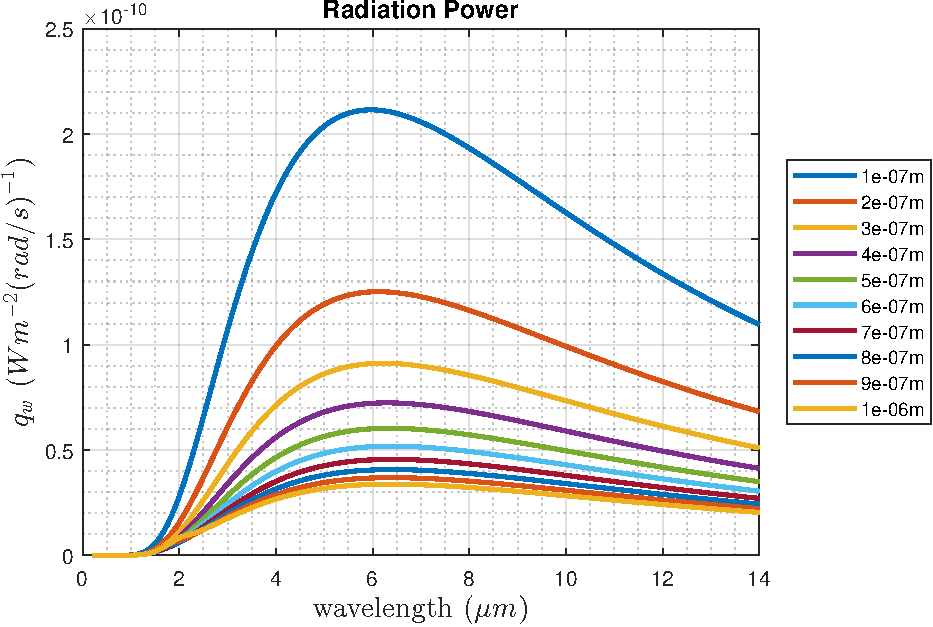
\includegraphics[width=1.00\textwidth]{figuras/Resultados/radiacion/SsGe.pdf}
	\caption{Potencia monocromática}
	\label{fig:SsGe}
\end{subfigure}
\begin{subfigure}[b]{0.49\textwidth}
	\centering
		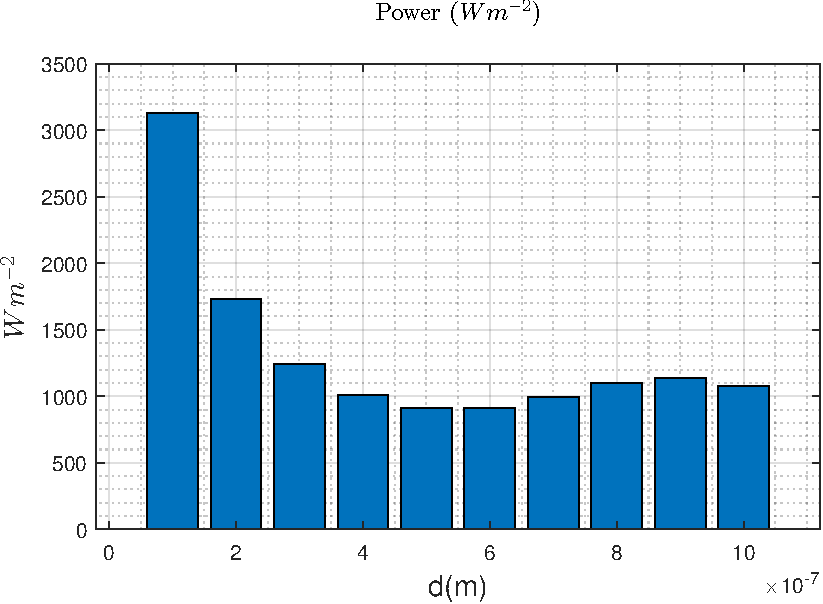
\includegraphics[width=1.00\textwidth]{figuras/Resultados/radiacion/p_Eg_SsGe.pdf}
	\caption{Potencia hasta 0.7 eV}
	\label{fig:p_Eg_SsGe}
\end{subfigure}
\caption{(\subref{fig:SsGe}) Potencia radiada monocromática por campo cercano para un emisor de $SS$ y una célula de $Ge$. (\subref{fig:p_Eg_SsGe}) Potencia radiada para un rango de longitudes de onda cuya energía es mayor a los 0.7eV ($\sim 1.8 \ \mu m$).}
	\label{fig:rad_SsGe}
\end{figure}
Las potencias por unidad de área se encuentran en general en el rango de los miles de $W/m^2$, siendo inferior a la del $Si$ pero no por un factor de magnitud.
\begin{table}[H]
	\centering
		\begin{tabular}{|c||c|c|c|c||c|}
		\hline
		\multirow{2}{*}{ }& \multicolumn{5}{c|}{\textbf{\large Potencias según transmisión del calor}}\\ \cline{2-6}
& \multicolumn{4}{c||}{Conducción (W/nº esp.)}& Radiación $(W/m^2)$\\ \hline
Dist. (nm)&$P_{Normal}$&$P_{R_c-Cal.Max}$&$P_{R_c-Cal.Inter}$&$P_{R_c-Empirico}$&$P_{Eg>0.7eV}$\\ \hline \hline
100&4,80E-02&1,26815E-06&2,53438E-06&1,68E-03&3,13E+03\\ \hline 
200&3,42E-02&1,26813E-06&2,53431E-06&1,65E-03&1,73E+03\\ \hline 
300&2,64E-02&1,26811E-06&2,53424E-06&1,62E-03&1,24E+03\\ \hline 
400&2,15E-02&1,26809E-06&2,53417E-06&1,60E-03&1,01E+03\\ \hline 
500&1,81E-02&1,26808E-06&2,53410E-06&1,57E-03&9,11E+02\\ \hline 
600&1,56E-02&1,26806E-06&2,53403E-06&1,54E-03&9,10E+02\\ \hline 
700&1,37E-02&1,26804E-06&2,53396E-06&1,52E-03&9,93E+02\\ \hline 
800&1,22E-02&1,26802E-06&2,53388E-06&1,50E-03&1,10E+03\\ \hline 
900&1,11E-02&1,26800E-06&2,53381E-06&1,48E-03&1,14E+03\\ \hline 
1000&1,01E-02&1,26799E-06&2,53374E-06&1,45E-03&1,08E+03\\ \hline 
		\end{tabular}
	\caption{Tabla de recopilación de los resultados de las simulaciones de transmisión de calor por conducción y radiación de campo cercano para una nTPV de emisor de $SS$.}
	\label{tab:SsSiO2Ge}
\end{table}
 Se recopilan los resultados de las simulaciones en la tabla \ref{tab:SsSiO2Ge} y se observa que para un centímetro cuadrado de superficie de radiación las potencias se encuentran en el rango de los 0.1 $W$, no siendo suficientemente mayor para que para un nano-espaciador la relación de las potencias para todas las distancias sea $\sim$10 (figura \ref{fig:rel_SsSiO2Ge}), pero para los casos con resistencia de contacto sí que se cumple. 
\begin{figure}[H]
	\centering
	\begin{subfigure}[b]{0.49\textwidth}
		\centering
			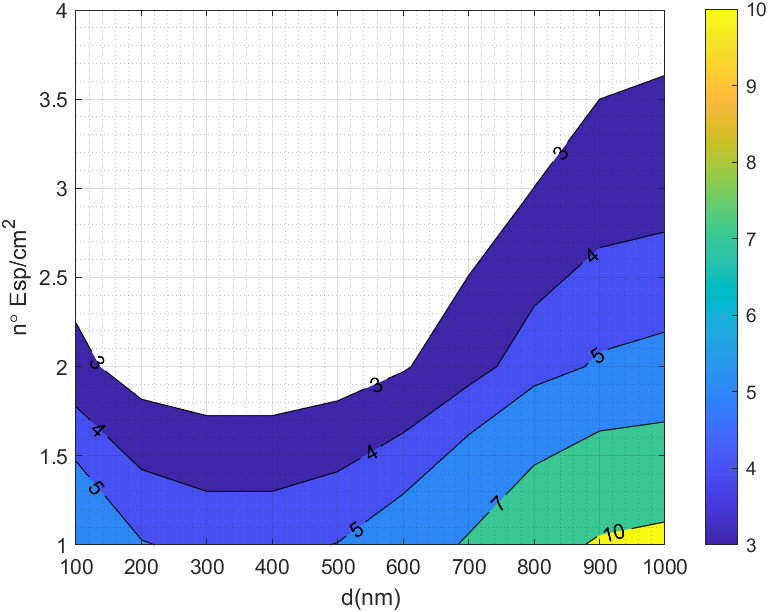
\includegraphics[width=1.00\textwidth]{figuras/Resultados/RelacionCondRad/SS.png}
		\caption{Sin $R_c$}
		\label{fig:rel_SsSiO2Ge}
	\end{subfigure}
	\hfill
	\begin{subfigure}[b]{0.49\textwidth}
		\centering
			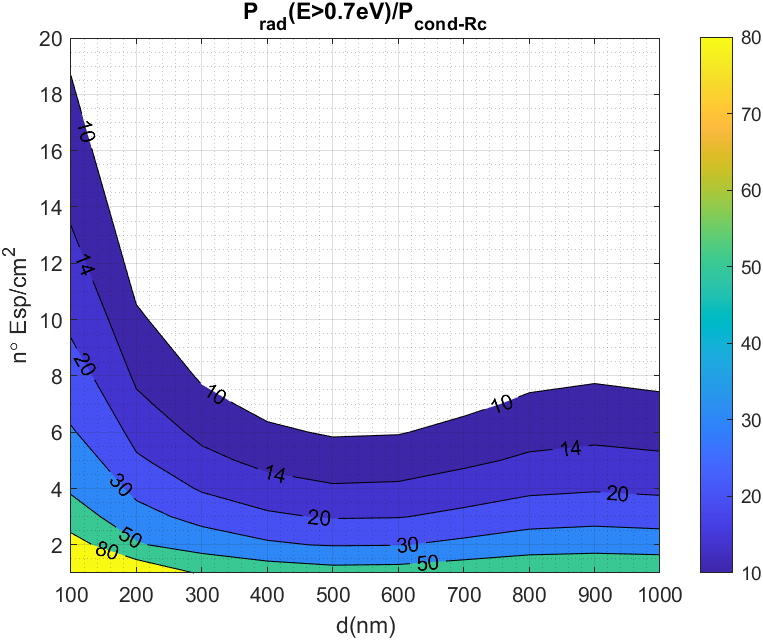
\includegraphics[width=1.00\textwidth]{figuras/Resultados/RelacionCondRad/SS_Rc_empirico.png}
		\caption{$R_c$ empírica}
		\label{fig:rel_SsSiO2Ge_Rc_emp}
	\end{subfigure}
	\hfill
	\begin{subfigure}[b]{0.49\textwidth}
		\centering
			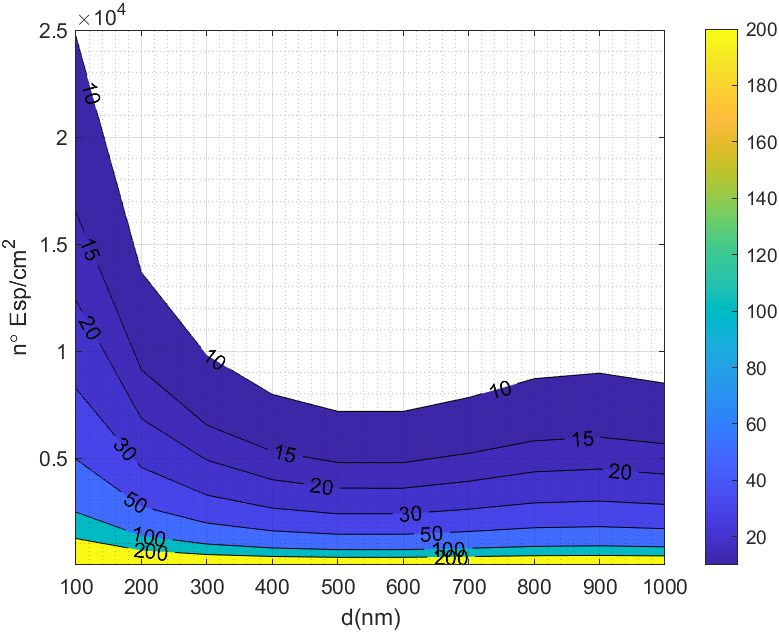
\includegraphics[width=1.00\textwidth]{figuras/Resultados/RelacionCondRad/SS_Rc.png}
		\caption{$R_c$ calculada máxima}
		\label{fig:rel_SsSiO2Ge_Rc_max}
	\end{subfigure}
	\hfill
	\begin{subfigure}[b]{0.49\textwidth}
		\centering
			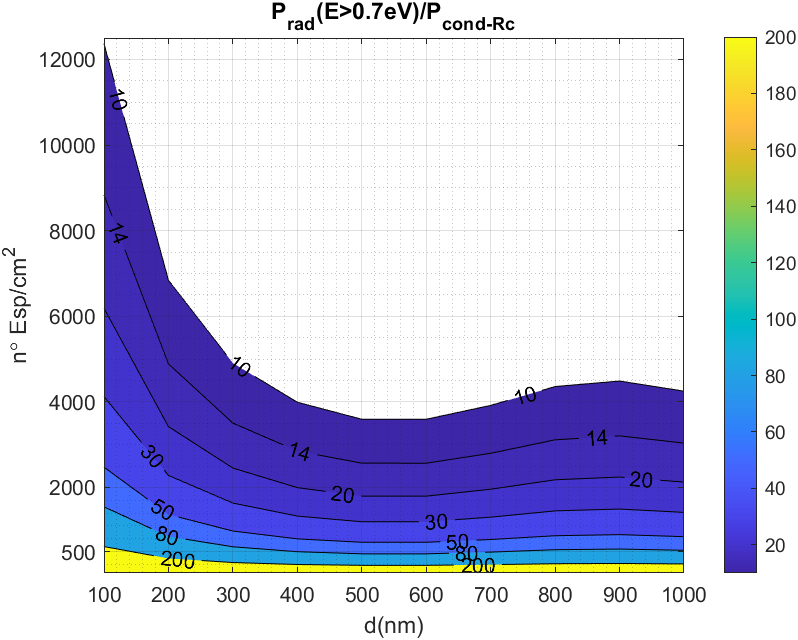
\includegraphics[width=1.00\textwidth]{figuras/Resultados/RelacionCondRad/SS_Rc_Intermedio.png}
		\caption{$R_c$ calculada intermedia}
		\label{fig:rel_SsSiO2Ge_Rc_inter}
	\end{subfigure}
	\caption[Relación de las potencias de conducción y radiación para un emisor de $SS$ según el número de nano-espaciadores y la altura de los nano-espaciadores para un emisor y célula de 1 $cm^2$]{Relación de las potencias de conducción y radiación para un emisor de $SS$ según el número de nano-espaciadores y la altura de los nano-espaciadores para un emisor y célula de 1 $cm^2$. (\subref{fig:rel_SsSiO2Ge}) Relación de potencias sin $R_c$. (\subref{fig:rel_SsSiO2Ge_Rc_emp}) Relación de potencias con $R_c$ empírica \cite{nf_TPV_Pillars_SiO2}. (\subref{fig:rel_SsSiO2Ge_Rc_max}) Relación de potencias con $R_c$ calculada máxima. (\subref{fig:rel_SsSiO2Ge_Rc_inter}) Relación de potencias con $R_c$ calculada intermedia. }
	\label{fig:relation_SsSiO2Ge}
\end{figure}
Para el caso que la $R_c$ empírica la cantidad máxima de nano-espaciadores para una relación de $\sim$10 entre las potencias no supera los 20 nano-espaciadores (figura \ref{fig:rel_SsSiO2Ge_Rc_emp}), a diferencia del nTPV con emisor de $Si$ que casi llega a los 30 nano-espaciadores (figura \ref{fig:rel_SiSiO2Ge_Rc}).\\\\
Para el resto de casos de $R_c$ la cantidad de nano-espaciadores para tener una relación de mínimo 10 supera la cantidad de mil, lo que implica que al disminuir el número de nano-espaciadores aumenta considerablemente la relación entre las potencias de conducción y radiación, siendo aproximadamente unos 2500 y 1000 nano-espaciadores para la $R_c$ máxima y la $R_c$ intermedia, respectivamente.
%%%%%%%%%%%    SiC-SiO2-Ge
\section{Resultados de las simulaciones para una nTPV de SiC-SiO2-Ge}
Se procede a estudiar el caso para un emisor de Carburo de Silicio ($SiC$) por ser una material con mayor conductividad térmica a 800\textdegree C que para un emisor de $Si$ y $SS$, cuyas conductividades térmicas a 800\textdegree C ronda entre los 26 y 30 $W/(m^2 K)$ a diferencia del $SiC$ que ronda los 60 $W/(m^2 K)$. Además el $SiC$ tiene un punto de fusión mayor que el $Si$ y el $SS$, siendo una característica del material de gran utilidad para su uso en baterías que almacenan la energía en forma de calor.\\\\
A su vez el $SiC$ ha sido usado en \cite{doi:Near_field_ThinFilm}, que mediante una capa fina de $SiC$ depositada en el emisor se aumentó de flujo de calor por radiación de campo cercano entre el emisor y el receptor de $SiC$.
\begin{figure}[H]
	\centering
	\begin{subfigure}[b]{0.49\textwidth}
		\centering
			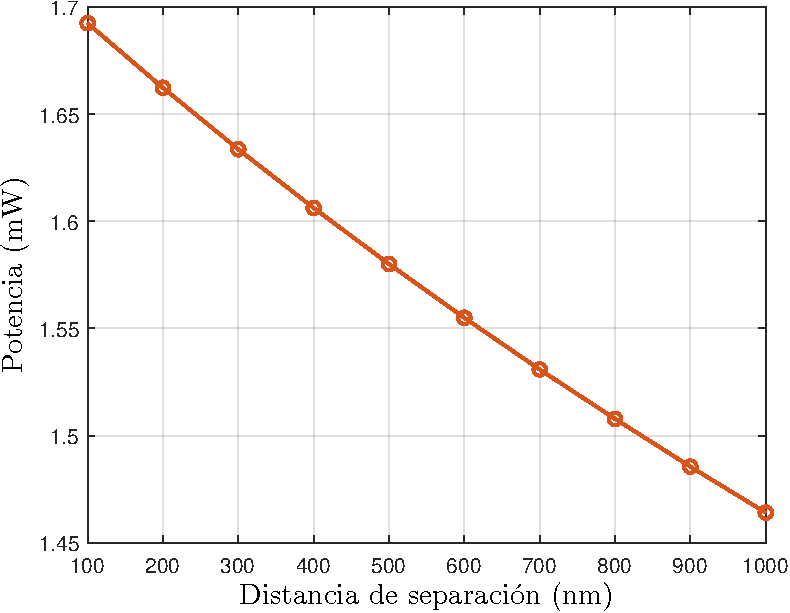
\includegraphics[width=1\textwidth]{figuras/Resultados/conduccion/pdf/Prc_SiCSiO2Ge.pdf}
		\caption{Potencias de conducción}
		\label{fig:Prc_SiCSiO2Ge}
	\end{subfigure}
	\hfill
	\begin{subfigure}[b]{0.49\textwidth}
		\centering
			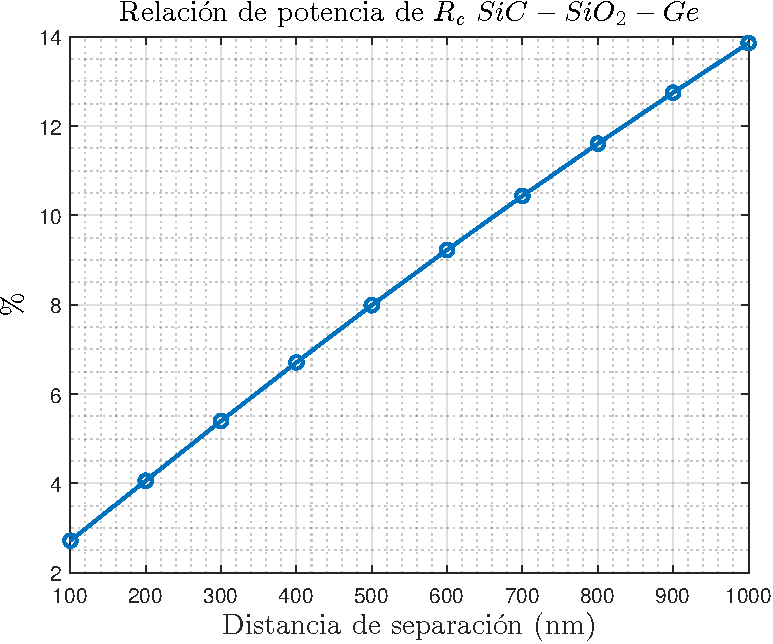
\includegraphics[width=0.9\textwidth]{figuras/Resultados/conduccion/pdf/relPrc_SiCSiO2Ge.pdf}
		\caption{Relación de potencia $R_c$}
		\label{fig:relPrc_SiCSiO2Ge}
	\end{subfigure}
	\caption{(\subref{fig:Prc_SiCSiO2Ge}) Potencias de conducción para sin y con el efecto de la $R_c$ empírica, eje izquierdo para el caso sin $R_c$ y eje derecho para el caso con $R_c$. (\subref{fig:relPrc_SiCSiO2Ge}) Relación de la potencia de conducción con $R_c$ respecto a sin $R_c$.}
	\label{fig:PrcCond_SiCSiO2Ge}
\end{figure}
Se realizan las simulaciones de transmisión de calor por conducción, obteniéndose resultados similares a los casos anteriores porque la mayor cantidad de caída de temperatura se produce en el nano-espaciador por tener una baja conductividad térmica respecto al emisor y la célula. Algo que si se nota es que la potencia máxima es $\sim 0.85\cdot 10^{-2}$ W mayor que para el emisor de $Si$ pero la relación entre las potencias con $R_c$ respecto a sin $R_c$ es menor, no superando el 14\% como valor máximo a los 1000nm.\\\\
Para las simulaciones de transmisión de calor por radiación de campo cercano se obtienen curvas de potencias monocromáticas por unidad de área muy parecidas a las del emisor de $Si$ para las longitudes de onda más pequeñas o de alta energía, obteniéndose valores de potencia por unidad de área similares.
\begin{figure}[h]
	\centering
		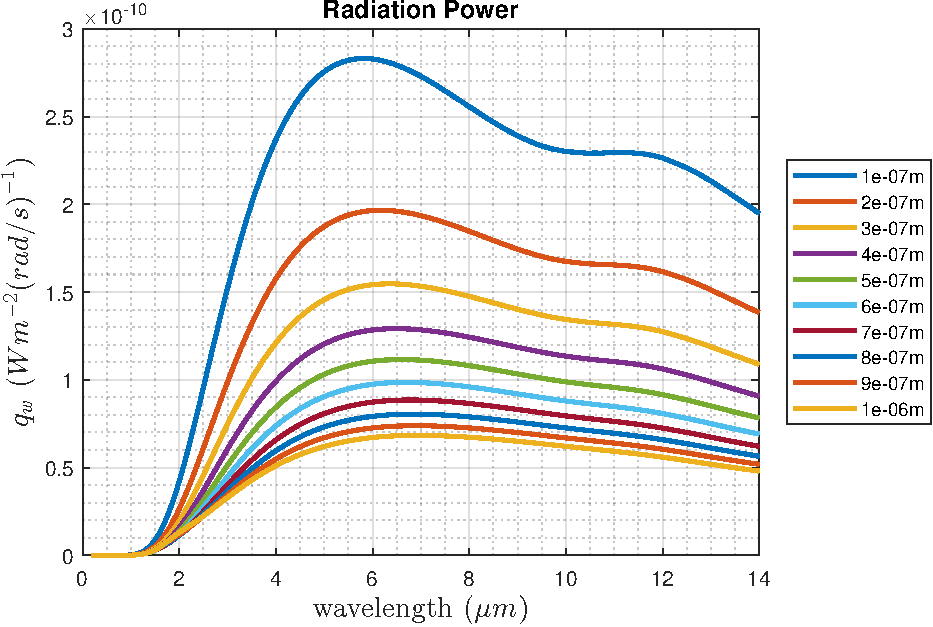
\includegraphics[width=1.00\textwidth]{figuras/Resultados/radiacion/SiCGe.pdf}
	\caption{ }
	\label{fig:rad_SiCGe}
\end{figure}


\begin{table}[h]
	\centering
		\begin{tabular}{|c||c|c||c|c|}
		\hline
\multirow{2}{*}{ }& \multicolumn{4}{c|}{\textbf{\large Potencias según transmisión del calor}}\\ \cline{2-5}
& \multicolumn{2}{c||}{Conducción (W/nº esp.)}& \multicolumn{2}{c|}{Radiación $(W/m^2)$}\\ \hline
Dist. (nm)&$P_{Normal}$&$P_{R_c-Empirico}$&$P_{Eg>0.7eV}$&$P_{full}$\\ \hline \hline
100&6,23E-02&1,69E-03&4,90E+03&1,50E+05\\ \hline 
200&4,09E-02&1,66E-03&3,00E+03&1,01E+05\\ \hline 
300&3,03E-02&1,63E-03&2,21E+03&7,80E+04\\ \hline 
400&2,39E-02&1,61E-03&1,82E+03&6,43E+04\\ \hline 
500&1,98E-02&1,58E-03&1,64E+03&5,52E+04\\ \hline 
600&1,68E-02&1,55E-03&1,60E+03&4,87E+04\\ \hline 
700&1,47E-02&1,53E-03&1,67E+03&4,40E+04\\ \hline 
800&1,30E-02&1,51E-03&1,76E+03&4,06E+04\\ \hline 
900&1,17E-02&1,49E-03&1,81E+03&3,80E+04\\ \hline 
1000&1,06E-02&1,46E-03&1,75E+03&3,61E+04\\ \hline 
		\end{tabular}
	\caption{dac}
	\label{tab:dac}
\end{table}

relleno


\begin{figure}[H]
	\centering
	%% Si-SiO2-Si Eg
	\begin{subfigure}[b]{0.49\textwidth}
		\centering
		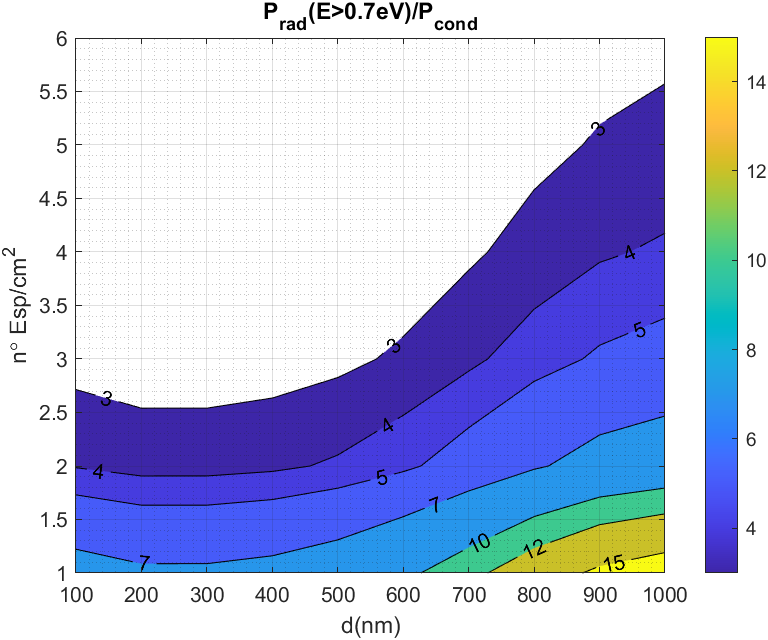
\includegraphics[width=1.00\textwidth]{figuras/Resultados/RelacionCondRad/SiC_Ge.png}
		\caption{ }
		\label{fig:rel_SiCSiO2Ge}
	\end{subfigure}
	\hfill
	\begin{subfigure}[b]{0.49\textwidth}
		\centering
		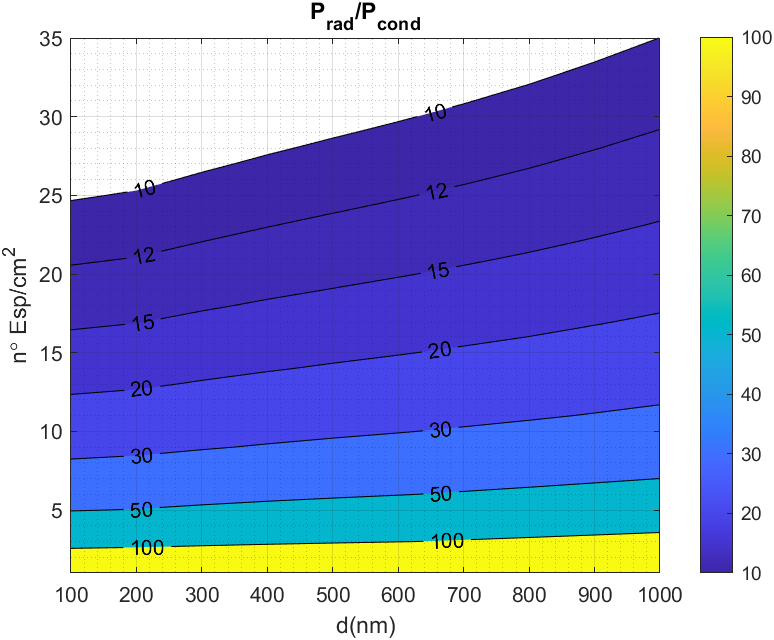
\includegraphics[width=1.00\textwidth]{figuras/Resultados/RelacionCondRad/SiC_Ge_full.png}
		\caption{ }
		\label{fig:rel_SiCSiO2Ge_Rc}
	\end{subfigure}
	\hfill
	\begin{subfigure}[b]{0.49\textwidth}
		\centering
		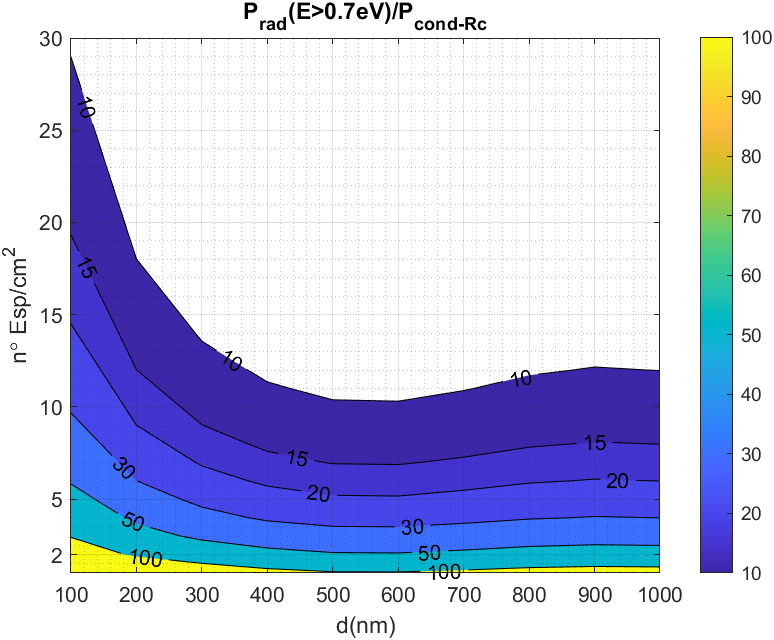
\includegraphics[width=1.00\textwidth]{figuras/Resultados/RelacionCondRad/SiC_Rc.png}
		\caption{ }
		\label{fig:rel_SiCSiO2Ge_full}
	\end{subfigure}
	\hfill
	\begin{subfigure}[b]{0.49\textwidth}
		\centering
		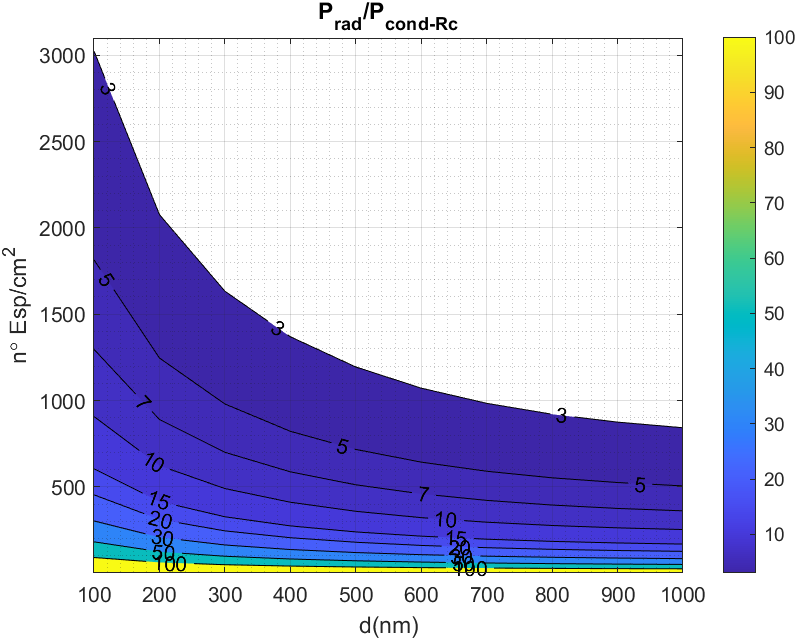
\includegraphics[width=1.00\textwidth]{figuras/Resultados/RelacionCondRad/SiC_Ge_Rc_full.png}
		\caption{ }
		\label{fig:rel_SiCSiO2Ge_Rc_full}
	\end{subfigure}
	\caption{ }
	\label{fig:relation_SiCSiO2Ge}
\end{figure}
\section{Número de nano-espaciadores para soportar la carga}
\section{Resultados de las simulaciones para una nTPV de Si-Si-Ge y SS-Si-Ge}
%% comparar el efecto de cambiar el material del nano-espaciador
\begin{table}[H]
	\centering
		\begin{tabular}{|c|c|c|}
		\hline
		dnm&Prcpaper&Prc\_SS\\ \hline 
		100&0,0017136&0,00171126\\ \hline 
		200&0,0017135&0,00171117\\ \hline 
		300&0,00171336&0,00171103\\ \hline 
		400&0,00171322&0,00171089\\ \hline 
		500&0,00171304&0,00171072\\ \hline 
		600&0,00171282&0,0017105\\ \hline 
		700&0,00171257&0,00171025\\ \hline 
		800&0,0017125&0,00171019\\ \hline 
		900&0,0017122&0,00170989\\ \hline 
		1000&0,00171208&0,00170978\\ \hline
		\end{tabular}
	\caption{nano-espaciador de Si}
	\label{tab:nanoEspaciadorDeSi}
\end{table}
\begin{figure}[H]
	\centering
		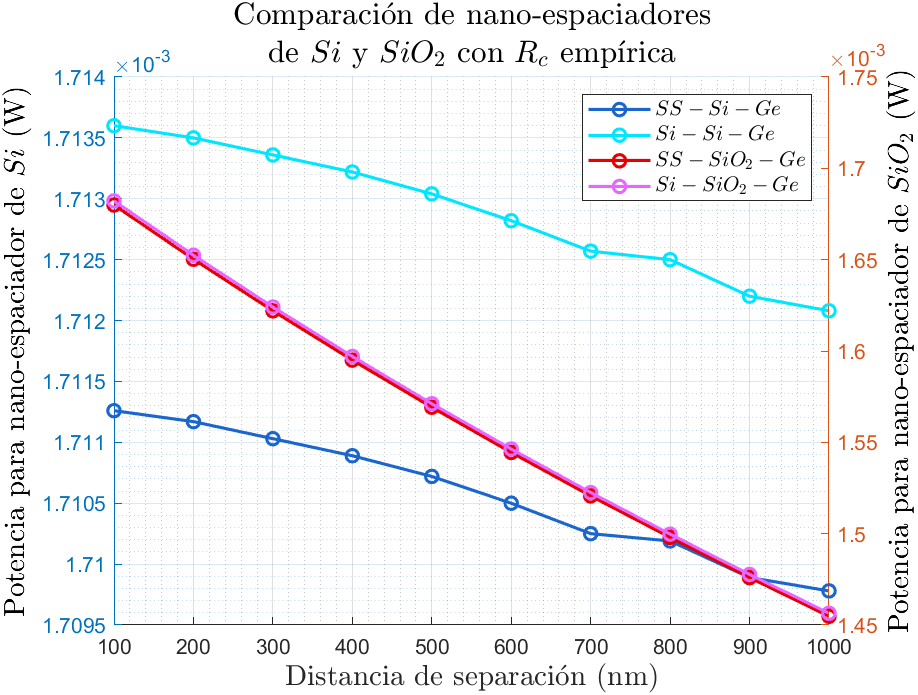
\includegraphics[width=0.6\textwidth]{figuras/Resultados/conduccion/relaciones_SiySiO2.png}
	\caption{ }
	\label{fig:relaciones_SiySiO2}
\end{figure}

\section{Discusión}